\batchmode
\documentclass[spanish,a4paper,12pt,twoside]{report}
\RequirePackage{ifthen}




\usepackage[dvips]{graphicx}
\usepackage[dvips]{epsfig}
\usepackage[latin1]{inputenc}
\usepackage[spanish]{babel}
\usepackage{alltt}
\usepackage{algorithm}
\usepackage{algorithmic}
\usepackage{multirow}
\usepackage{hyperref}


\makeatletter
\let\orgdescriptionlabel\let\orglabel\label
  \let\label\@gobble
  \phantomsection
  \edef \@currentlabel{%
\renewcommand }\let\label\orglabel
  \orgdescriptionlabel{%
\renewcommand }{descriptionlabel}[1]{%
  \let\orglabel\label
  \let\label\@gobble
  \phantomsection
  \edef \@currentlabel{#1}%
  \let\label\orglabel
  \orgdescriptionlabel{#1}%
}
\makeatother


\usepackage{makeidx}
\makeindex


\usepackage{listings}
\lstset{language=Ruby}
\lstset{
  showstringspaces=false
  escapeinside={\#(*}{*)},
  numbers=left,
  basicstyle=\footnotesize
}


\usepackage[official]{eurosym}

%
\providecommand{\SONY}{{\sc Sony}}%
\providecommand{\MICROSOFT}{{\sc Microsoft}}%
\providecommand{\GCC}{\textsf{\textsc{G}CC}}%
\providecommand{\INTEL}{\textsf{\textsc{I}ntel}} 


%
\renewcommand{\algorithmicwhile}{\textbf{mientras}}
%
\renewcommand{\algorithmicend}{\textbf{fin}}
%
\renewcommand{\algorithmicdo}{\textbf{hacer}}
%
\renewcommand{\algorithmicif}{\textbf{si}}
%
\renewcommand{\algorithmicthen}{\textbf{entonces}}
%
\renewcommand{\algorithmicrepeat}{\textbf{repetir}}
%
\renewcommand{\algorithmicuntil}{\textbf{hasta que}}
%
\renewcommand{\algorithmicelse}{\textbf{en otro caso}}
%
\renewcommand{\algorithmicfor}{\textbf{para}}

%
\providecommand{\RET}{\STATE \textbf{retornar} }%
\providecommand{\TO}{\textbf{hasta} }%
\providecommand{\AND}{\textbf{y} }%
\providecommand{\OR}{\textbf{o} } 

%
\providecommand{\cei}[1]{\index{#1}\emph{#1}} 

%
\providecommand{\ceis}[1]{\index{#1}{\bfseries {#1}}} 

%
\providecommand{\ceit}[1]{\index{#1}{#1}} 



%
\newenvironment{sourcecode}{\begin{list}{}{\setlength{\leftmargin}{1em}}\item\scriptsize\bfseries}
{\end{list}} 



%
\newenvironment{littlesourcecode}{\begin{list}{}{\setlength{\leftmargin}{1em}}\item\tiny\bfseries}
{\end{list}} 



%
\newenvironment{summary}{

\noindent\begin{center}\textbf{Abstract}\end{center}\begin{itshape}

\noindent}
{\end{itshape}} 



%
\newenvironment{keywords}{\begin{list}{}{\setlength{\leftmargin}{1em}}\item[\hskip\labelsep \bfseries Keywords:]}
{\end{list}} 



%
\newenvironment{palabrasClave}{\begin{list}{}{\setlength{\leftmargin}{1em}}\item[\hskip\labelsep \bfseries Palabras clave:]}
{\end{list}} 


\oddsidemargin 5 mm
\evensidemargin 5 mm


\textwidth 15 cm


\input{amssym.def}




\usepackage[dvips]{color}


\pagecolor[gray]{.7}

\usepackage[latin1]{inputenc}



\makeatletter

\makeatletter
\count@=\the\catcode`\_ \catcode`\_=8 
\newenvironment{tex2html_wrap}{}{}%
\catcode`\<=12\catcode`\_=\count@
\newcommand{\providedcommand}[1]{\expandafter\providecommand\csname #1\endcsname}%
\newcommand{\renewedcommand}[1]{\expandafter\providecommand\csname #1\endcsname{}%
  \expandafter\renewcommand\csname #1\endcsname}%
\newcommand{\newedenvironment}[1]{\newenvironment{#1}{}{}\renewenvironment{#1}}%
\let\newedcommand\renewedcommand
\let\renewedenvironment\newedenvironment
\makeatother
\let\mathon=$
\let\mathoff=$
\ifx\AtBeginDocument\undefined \newcommand{\AtBeginDocument}[1]{}\fi
\newbox\sizebox
\setlength{\hoffset}{0pt}\setlength{\voffset}{0pt}
\addtolength{\textheight}{\footskip}\setlength{\footskip}{0pt}
\addtolength{\textheight}{\topmargin}\setlength{\topmargin}{0pt}
\addtolength{\textheight}{\headheight}\setlength{\headheight}{0pt}
\addtolength{\textheight}{\headsep}\setlength{\headsep}{0pt}
\setlength{\textwidth}{349pt}
\newwrite\lthtmlwrite
\makeatletter
\let\realnormalsize=\normalsize
\global\topskip=2sp
\def\preveqno{}\let\real@float=\@float \let\realend@float=\end@float
\def\@float{\let\@savefreelist\@freelist\real@float}
\def\liih@math{\ifmmode$\else\bad@math\fi}
\def\end@float{\realend@float\global\let\@freelist\@savefreelist}
\let\real@dbflt=\@dbflt \let\end@dblfloat=\end@float
\let\@largefloatcheck=\relax
\let\if@boxedmulticols=\iftrue
\def\@dbflt{\let\@savefreelist\@freelist\real@dbflt}
\def\adjustnormalsize{\def\normalsize{\mathsurround=0pt \realnormalsize
 \parindent=0pt\abovedisplayskip=0pt\belowdisplayskip=0pt}%
 \def\phantompar{\csname par\endcsname}\normalsize}%
\def\lthtmltypeout#1{{\let\protect\string \immediate\write\lthtmlwrite{#1}}}%
\newcommand\lthtmlhboxmathA{\adjustnormalsize\setbox\sizebox=\hbox\bgroup\kern.05em }%
\newcommand\lthtmlhboxmathB{\adjustnormalsize\setbox\sizebox=\hbox to\hsize\bgroup\hfill }%
\newcommand\lthtmlvboxmathA{\adjustnormalsize\setbox\sizebox=\vbox\bgroup %
 \let\ifinner=\iffalse \let\)\liih@math }%
\newcommand\lthtmlboxmathZ{\@next\next\@currlist{}{\def\next{\voidb@x}}%
 \expandafter\box\next\egroup}%
\newcommand\lthtmlmathtype[1]{\gdef\lthtmlmathenv{#1}}%
\newcommand\lthtmllogmath{\dimen0\ht\sizebox \advance\dimen0\dp\sizebox
  \ifdim\dimen0>.95\vsize
   \lthtmltypeout{%
*** image for \lthtmlmathenv\space is too tall at \the\dimen0, reducing to .95 vsize ***}%
   \ht\sizebox.95\vsize \dp\sizebox\z@ \fi
  \lthtmltypeout{l2hSize %
:\lthtmlmathenv:\the\ht\sizebox::\the\dp\sizebox::\the\wd\sizebox.\preveqno}}%
\newcommand\lthtmlfigureA[1]{\let\@savefreelist\@freelist
       \lthtmlmathtype{#1}\lthtmlvboxmathA}%
\newcommand\lthtmlpictureA{\bgroup\catcode`\_=8 \lthtmlpictureB}%
\newcommand\lthtmlpictureB[1]{\lthtmlmathtype{#1}\egroup
       \let\@savefreelist\@freelist \lthtmlhboxmathB}%
\newcommand\lthtmlpictureZ[1]{\hfill\lthtmlfigureZ}%
\newcommand\lthtmlfigureZ{\lthtmlboxmathZ\lthtmllogmath\copy\sizebox
       \global\let\@freelist\@savefreelist}%
\newcommand\lthtmldisplayA{\bgroup\catcode`\_=8 \lthtmldisplayAi}%
\newcommand\lthtmldisplayAi[1]{\lthtmlmathtype{#1}\egroup\lthtmlvboxmathA}%
\newcommand\lthtmldisplayB[1]{\edef\preveqno{(\theequation)}%
  \lthtmldisplayA{#1}\let\@eqnnum\relax}%
\newcommand\lthtmldisplayZ{\lthtmlboxmathZ\lthtmllogmath\lthtmlsetmath}%
\newcommand\lthtmlinlinemathA{\bgroup\catcode`\_=8 \lthtmlinlinemathB}
\newcommand\lthtmlinlinemathB[1]{\lthtmlmathtype{#1}\egroup\lthtmlhboxmathA
  \vrule height1.5ex width0pt }%
\newcommand\lthtmlinlineA{\bgroup\catcode`\_=8 \lthtmlinlineB}%
\newcommand\lthtmlinlineB[1]{\lthtmlmathtype{#1}\egroup\lthtmlhboxmathA}%
\newcommand\lthtmlinlineZ{\egroup\expandafter\ifdim\dp\sizebox>0pt %
  \expandafter\centerinlinemath\fi\lthtmllogmath\lthtmlsetinline}
\newcommand\lthtmlinlinemathZ{\egroup\expandafter\ifdim\dp\sizebox>0pt %
  \expandafter\centerinlinemath\fi\lthtmllogmath\lthtmlsetmath}
\newcommand\lthtmlindisplaymathZ{\egroup %
  \centerinlinemath\lthtmllogmath\lthtmlsetmath}
\def\lthtmlsetinline{\hbox{\vrule width.1em \vtop{\vbox{%
  \kern.1em\copy\sizebox}\ifdim\dp\sizebox>0pt\kern.1em\else\kern.3pt\fi
  \ifdim\hsize>\wd\sizebox \hrule depth1pt\fi}}}
\def\lthtmlsetmath{\hbox{\vrule width.1em\kern-.05em\vtop{\vbox{%
  \kern.1em\kern0.8 pt\hbox{\hglue.17em\copy\sizebox\hglue0.8 pt}}\kern.3pt%
  \ifdim\dp\sizebox>0pt\kern.1em\fi \kern0.8 pt%
  \ifdim\hsize>\wd\sizebox \hrule depth1pt\fi}}}
\def\centerinlinemath{%
  \dimen1=\ifdim\ht\sizebox<\dp\sizebox \dp\sizebox\else\ht\sizebox\fi
  \advance\dimen1by.5pt \vrule width0pt height\dimen1 depth\dimen1 
 \dp\sizebox=\dimen1\ht\sizebox=\dimen1\relax}

\def\lthtmlcheckvsize{\ifdim\ht\sizebox<\vsize 
  \ifdim\wd\sizebox<\hsize\expandafter\hfill\fi \expandafter\vfill
  \else\expandafter\vss\fi}%
\providecommand{\selectlanguage}[1]{}%
\makeatletter \tracingstats = 1 


\begin{document}
\pagestyle{empty}\thispagestyle{empty}\lthtmltypeout{}%
\lthtmltypeout{latex2htmlLength hsize=\the\hsize}\lthtmltypeout{}%
\lthtmltypeout{latex2htmlLength vsize=\the\vsize}\lthtmltypeout{}%
\lthtmltypeout{latex2htmlLength hoffset=\the\hoffset}\lthtmltypeout{}%
\lthtmltypeout{latex2htmlLength voffset=\the\voffset}\lthtmltypeout{}%
\lthtmltypeout{latex2htmlLength topmargin=\the\topmargin}\lthtmltypeout{}%
\lthtmltypeout{latex2htmlLength topskip=\the\topskip}\lthtmltypeout{}%
\lthtmltypeout{latex2htmlLength headheight=\the\headheight}\lthtmltypeout{}%
\lthtmltypeout{latex2htmlLength headsep=\the\headsep}\lthtmltypeout{}%
\lthtmltypeout{latex2htmlLength parskip=\the\parskip}\lthtmltypeout{}%
\lthtmltypeout{latex2htmlLength oddsidemargin=\the\oddsidemargin}\lthtmltypeout{}%
\makeatletter
\if@twoside\lthtmltypeout{latex2htmlLength evensidemargin=\the\evensidemargin}%
\else\lthtmltypeout{latex2htmlLength evensidemargin=\the\oddsidemargin}\fi%
\lthtmltypeout{}%
\makeatother
\setcounter{page}{1}
\onecolumn

% !!! IMAGES START HERE !!!

{\newpage\clearpage
\lthtmlinlineA{tex2html_nomath_inline7501}%
\textquestiondown%
\lthtmlinlineZ
\lthtmlcheckvsize\clearpage}


%
\providecommand{\HRule}{\rule{\linewidth}{1mm}}%



\setlength{\parindent}{0mm}%

\setlength{\parindent}{0mm}


\setlength{\parskip}{0mm}%

\setlength{\parskip}{0mm}


\setlength{\parindent}{5mm}%

\setlength{\parindent}{5mm}

\renewcommand{\thepage}{\roman{page}}

\renewcommand{\thepage}{\arabic{page}}
\stepcounter{chapter}
\stepcounter{section}
\stepcounter{section}
{\newpage\clearpage
\lthtmlpictureA{tex2html_wrap11550}%

\includegraphics[width=0.6\textwidth]{images/fill_in1.eps}%
\lthtmlpictureZ
\lthtmlcheckvsize\clearpage}

{\newpage\clearpage
\lthtmlpictureA{tex2html_wrap11554}%

\includegraphics[width=1\textwidth]{images/fill_in2.eps}%
\lthtmlpictureZ
\lthtmlcheckvsize\clearpage}

{\newpage\clearpage
\lthtmlpictureA{tex2html_wrap11558}%
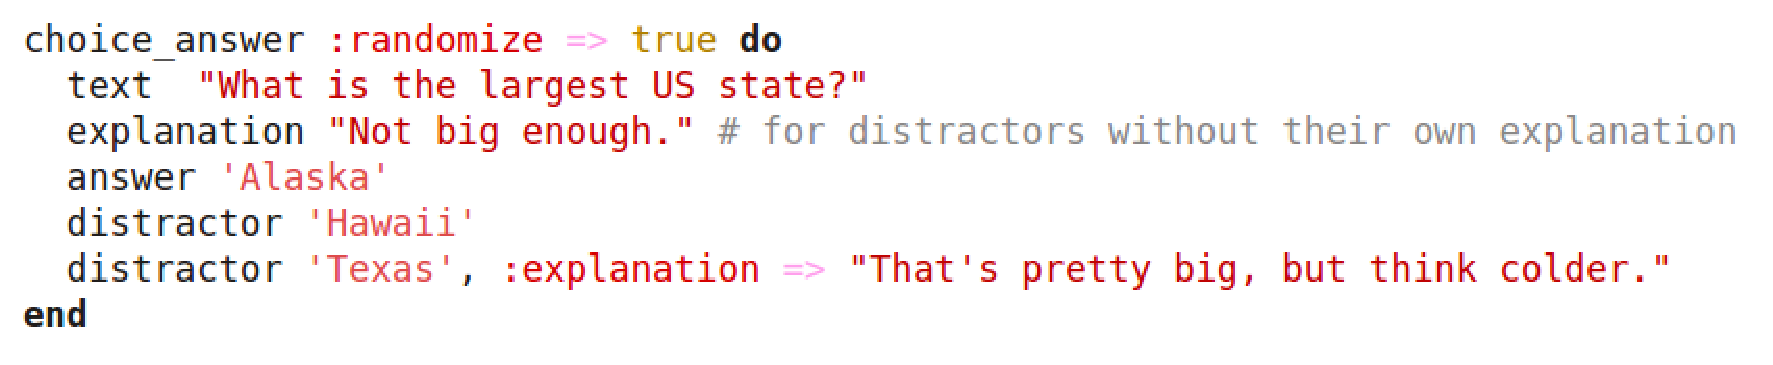
\includegraphics[width=1\textwidth]{images/choice_answer1.eps}%
\lthtmlpictureZ
\lthtmlcheckvsize\clearpage}

{\newpage\clearpage
\lthtmlpictureA{tex2html_wrap11562}%
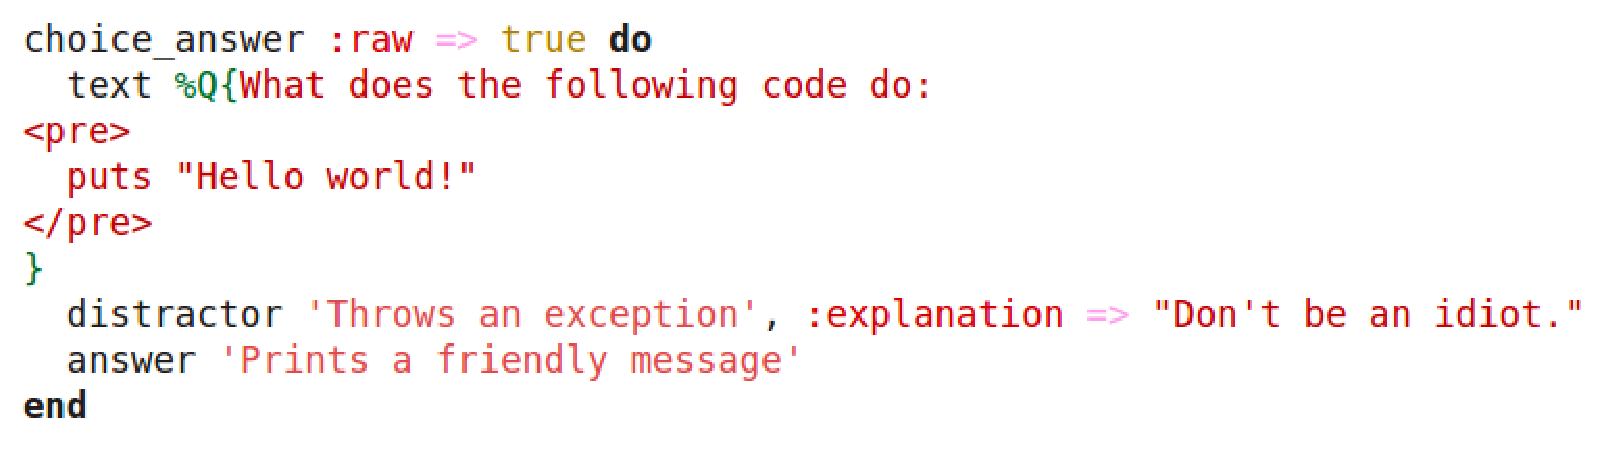
\includegraphics[width=0.9\textwidth]{images/choice_answer2.eps}%
\lthtmlpictureZ
\lthtmlcheckvsize\clearpage}

{\newpage\clearpage
\lthtmlpictureA{tex2html_wrap11566}%
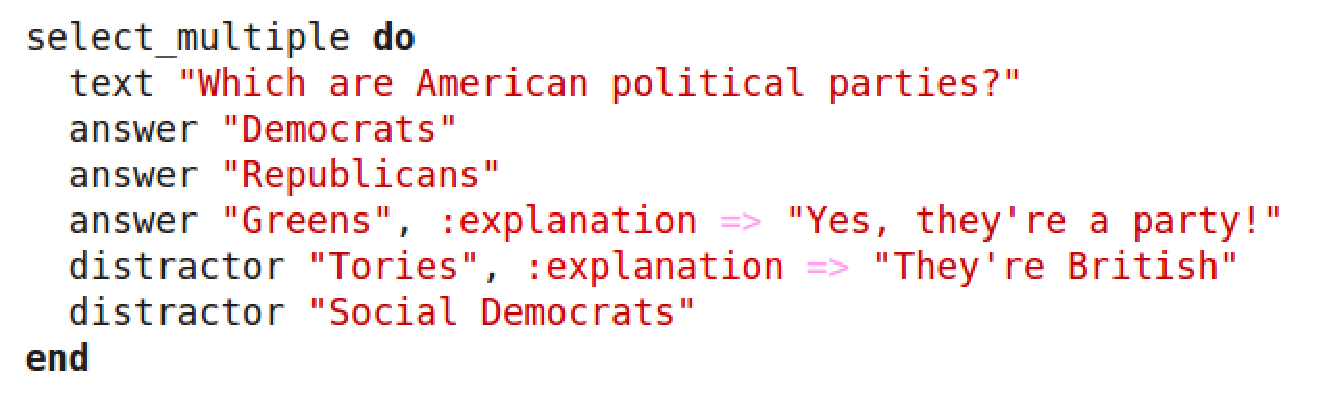
\includegraphics[width=0.8\textwidth]{images/select_multiple.eps}%
\lthtmlpictureZ
\lthtmlcheckvsize\clearpage}

{\newpage\clearpage
\lthtmlpictureA{tex2html_wrap11570}%
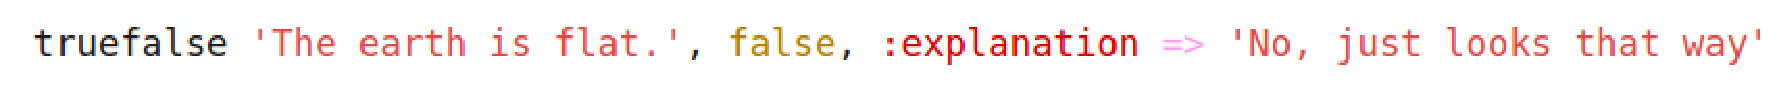
\includegraphics[width=1\textwidth]{images/truefalse.eps}%
\lthtmlpictureZ
\lthtmlcheckvsize\clearpage}

\stepcounter{subsection}
{\newpage\clearpage
\lthtmlfigureA{lstlisting947}%
\begin{lstlisting}
quiz 'Example quiz' do
\par
fill_in :points => 2 do
    text 'The capital of California is ---'
    answer 'sacramento'
  end
\par
choice_answer :randomize => true do
    text  "What is the largest US state?"
    explanation "Not big enough." # for distractors without their own explanation
    answer 'Alaska'
    distractor 'Hawaii'
    distractor 'Texas', :explanation => "That's pretty big, but think colder."
  end
\par
select_multiple do
    text "Which are American political parties?"
    answer "Democrats"
    answer "Republicans"
    answer "Greens", :explanation => "Yes, they're a party!"
    distractor "Tories", :explanation => "They're British"
    distractor "Social Democrats"
  end
\par
select_multiple do
    text "Which are American political parties?"
    answer "Democrats"
    answer "Republicans"
    answer "Greens", :explanation => "Yes, they're a party!"
    distractor "Tories", :explanation => "They're British"
    distractor "Social Democrats"
  end
\par
truefalse 'The week has 7 days.', true
  truefalse 'The earth is flat.', false, :explanation => 'No, just looks that way'
end
\end{lstlisting}%
\lthtmlfigureZ
\lthtmlcheckvsize\clearpage}

\stepcounter{section}
\stepcounter{section}
\stepcounter{section}
{\newpage\clearpage
\lthtmlpictureA{tex2html_wrap11577}%

\includegraphics{images/ruby.eps}%
\lthtmlpictureZ
\lthtmlcheckvsize\clearpage}

{\newpage\clearpage
\lthtmlpictureA{tex2html_wrap11578}%

\includegraphics[width=0.13\textwidth]{images/HTML5.eps}%
\lthtmlpictureZ
\lthtmlcheckvsize\clearpage}

{\newpage\clearpage
\lthtmlpictureA{tex2html_wrap11579}%

\includegraphics[width=0.1\textwidth]{images/css3.eps}%
\lthtmlpictureZ
\lthtmlcheckvsize\clearpage}

{\newpage\clearpage
\lthtmlpictureA{tex2html_wrap11580}%

\includegraphics[width=0.1\textwidth]{images/js.eps}%
\lthtmlpictureZ
\lthtmlcheckvsize\clearpage}

{\newpage\clearpage
\lthtmlpictureA{tex2html_wrap11581}%

\includegraphics[width=0.1\textwidth]{images/bootstrap.eps}%
\lthtmlpictureZ
\lthtmlcheckvsize\clearpage}

{\newpage\clearpage
\lthtmlpictureA{tex2html_wrap11582}%

\includegraphics[width=0.2\textwidth]{images/jquery.eps}%
\lthtmlpictureZ
\lthtmlcheckvsize\clearpage}

{\newpage\clearpage
\lthtmlpictureA{tex2html_wrap11583}%

\includegraphics[width=0.2\textwidth]{images/xregexp.eps}%
\lthtmlpictureZ
\lthtmlcheckvsize\clearpage}

{\newpage\clearpage
\lthtmlpictureA{tex2html_wrap11584}%

\includegraphics[width=0.2\textwidth]{images/mathjax.eps}%
\lthtmlpictureZ
\lthtmlcheckvsize\clearpage}

{\newpage\clearpage
\lthtmlpictureA{tex2html_wrap11585}%

\includegraphics[width=0.1\textwidth]{images/codemirror.eps}%
\lthtmlpictureZ
\lthtmlcheckvsize\clearpage}

{\newpage\clearpage
\lthtmlpictureA{tex2html_wrap11586}%

\includegraphics[width=0.1\textwidth]{images/mocha.eps}%
\lthtmlpictureZ
\lthtmlcheckvsize\clearpage}

{\newpage\clearpage
\lthtmlpictureA{tex2html_wrap11587}%

\includegraphics[width=0.1\textwidth]{images/chai.eps}%
\lthtmlpictureZ
\lthtmlcheckvsize\clearpage}

{\newpage\clearpage
\lthtmlpictureA{tex2html_wrap11588}%

\includegraphics[width=0.1\textwidth]{images/karma.eps}%
\lthtmlpictureZ
\lthtmlcheckvsize\clearpage}

{\newpage\clearpage
\lthtmlpictureA{tex2html_wrap11589}%

\includegraphics[width=0.1\textwidth]{images/sinatra.eps}%
\lthtmlpictureZ
\lthtmlcheckvsize\clearpage}

{\newpage\clearpage
\lthtmlpictureA{tex2html_wrap11590}%

\includegraphics[width=0.1\textwidth]{images/github.eps}%
\lthtmlpictureZ
\lthtmlcheckvsize\clearpage}

{\newpage\clearpage
\lthtmlpictureA{tex2html_wrap11591}%

\includegraphics[width=0.1\textwidth]{images/heroku.eps}%
\lthtmlpictureZ
\lthtmlcheckvsize\clearpage}

{\newpage\clearpage
\lthtmlpictureA{tex2html_wrap11592}%

\includegraphics[width=0.1\textwidth]{images/oauth.eps}%
\lthtmlpictureZ
\lthtmlcheckvsize\clearpage}

{\newpage\clearpage
\lthtmlpictureA{tex2html_wrap11593}%

\includegraphics[width=0.1\textwidth]{images/google_drive.eps}%
\lthtmlpictureZ
\lthtmlcheckvsize\clearpage}

\stepcounter{chapter}
\stepcounter{section}
\stepcounter{subsection}
{\newpage\clearpage
\lthtmlpictureA{tex2html_wrap11601}%
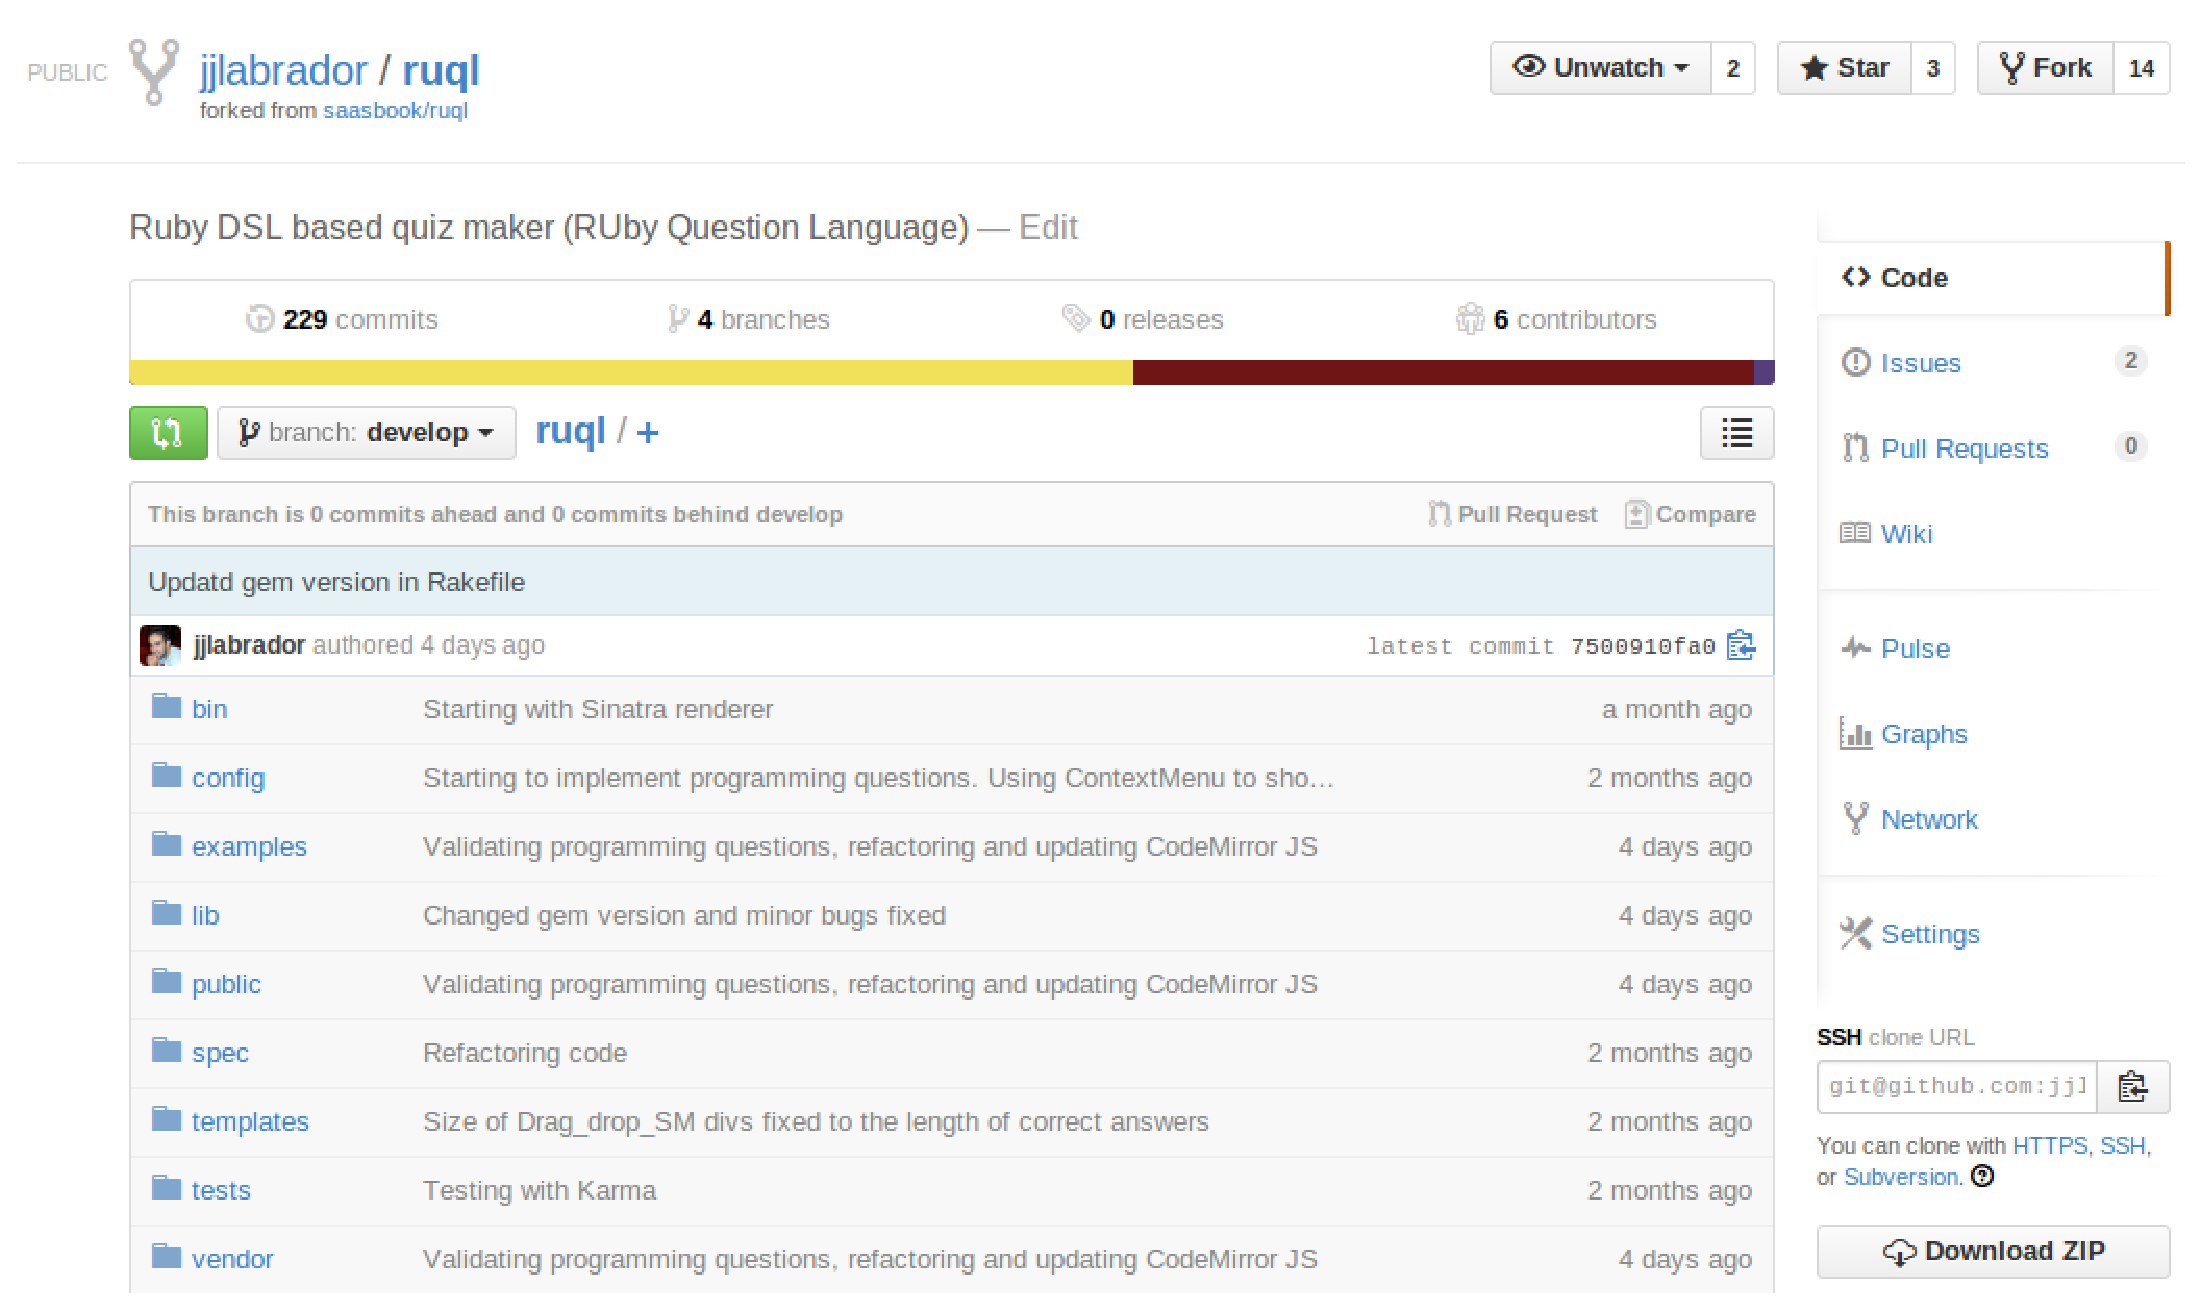
\includegraphics[width=\textwidth,height=0.58\textwidth]{images/github1.eps}%
\lthtmlpictureZ
\lthtmlcheckvsize\clearpage}

{\newpage\clearpage
\lthtmlpictureA{tex2html_wrap11605}%
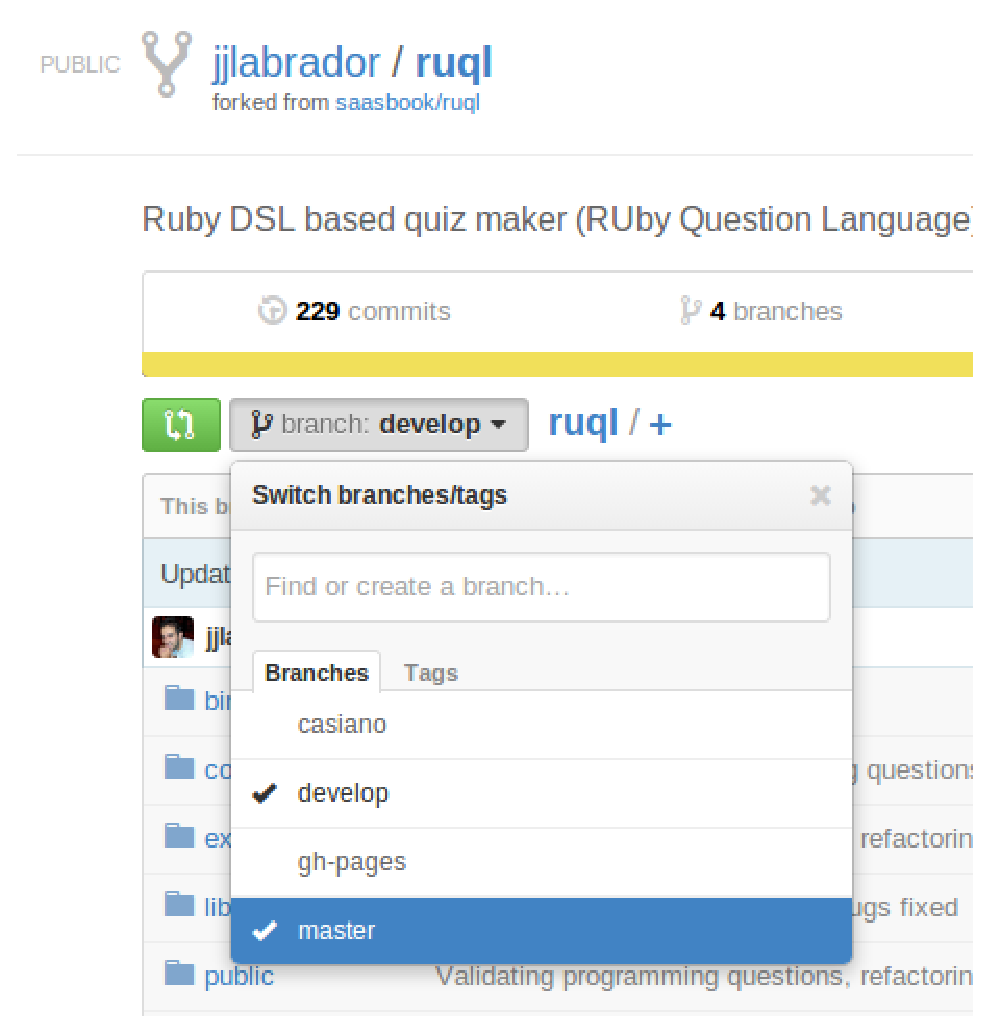
\includegraphics[width=0.47\textwidth]{images/github5.eps}%
\lthtmlpictureZ
\lthtmlcheckvsize\clearpage}

{\newpage\clearpage
\lthtmlpictureA{tex2html_wrap11609}%

\includegraphics[width=1\textwidth]{images/github2.eps}%
\lthtmlpictureZ
\lthtmlcheckvsize\clearpage}

{\newpage\clearpage
\lthtmlpictureA{tex2html_wrap11613}%
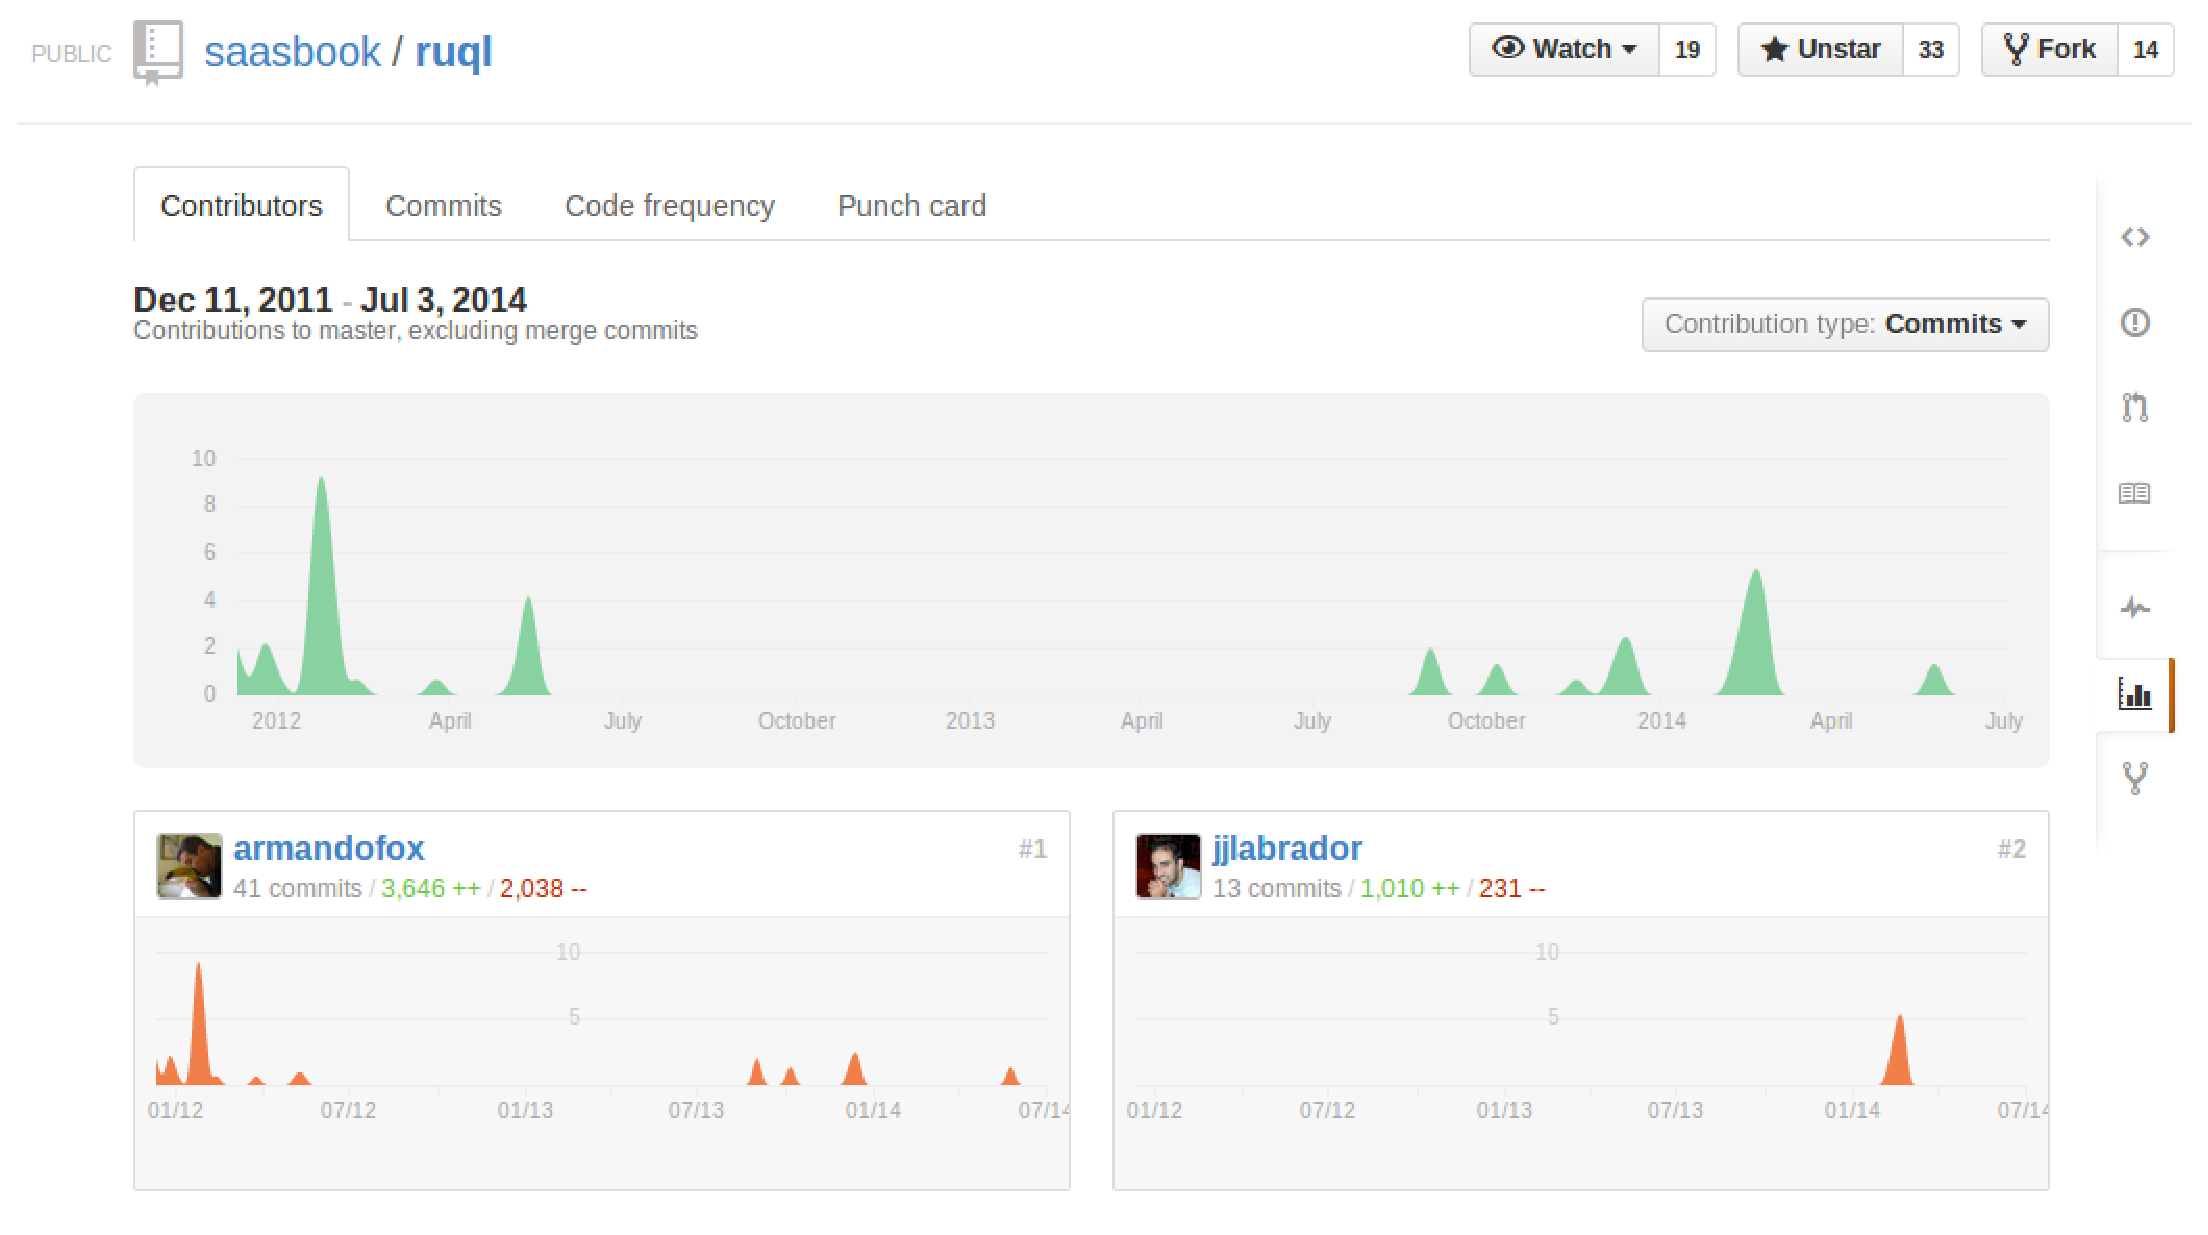
\includegraphics[width=1\textwidth]{images/github3.eps}%
\lthtmlpictureZ
\lthtmlcheckvsize\clearpage}

{\newpage\clearpage
\lthtmlpictureA{tex2html_wrap11617}%
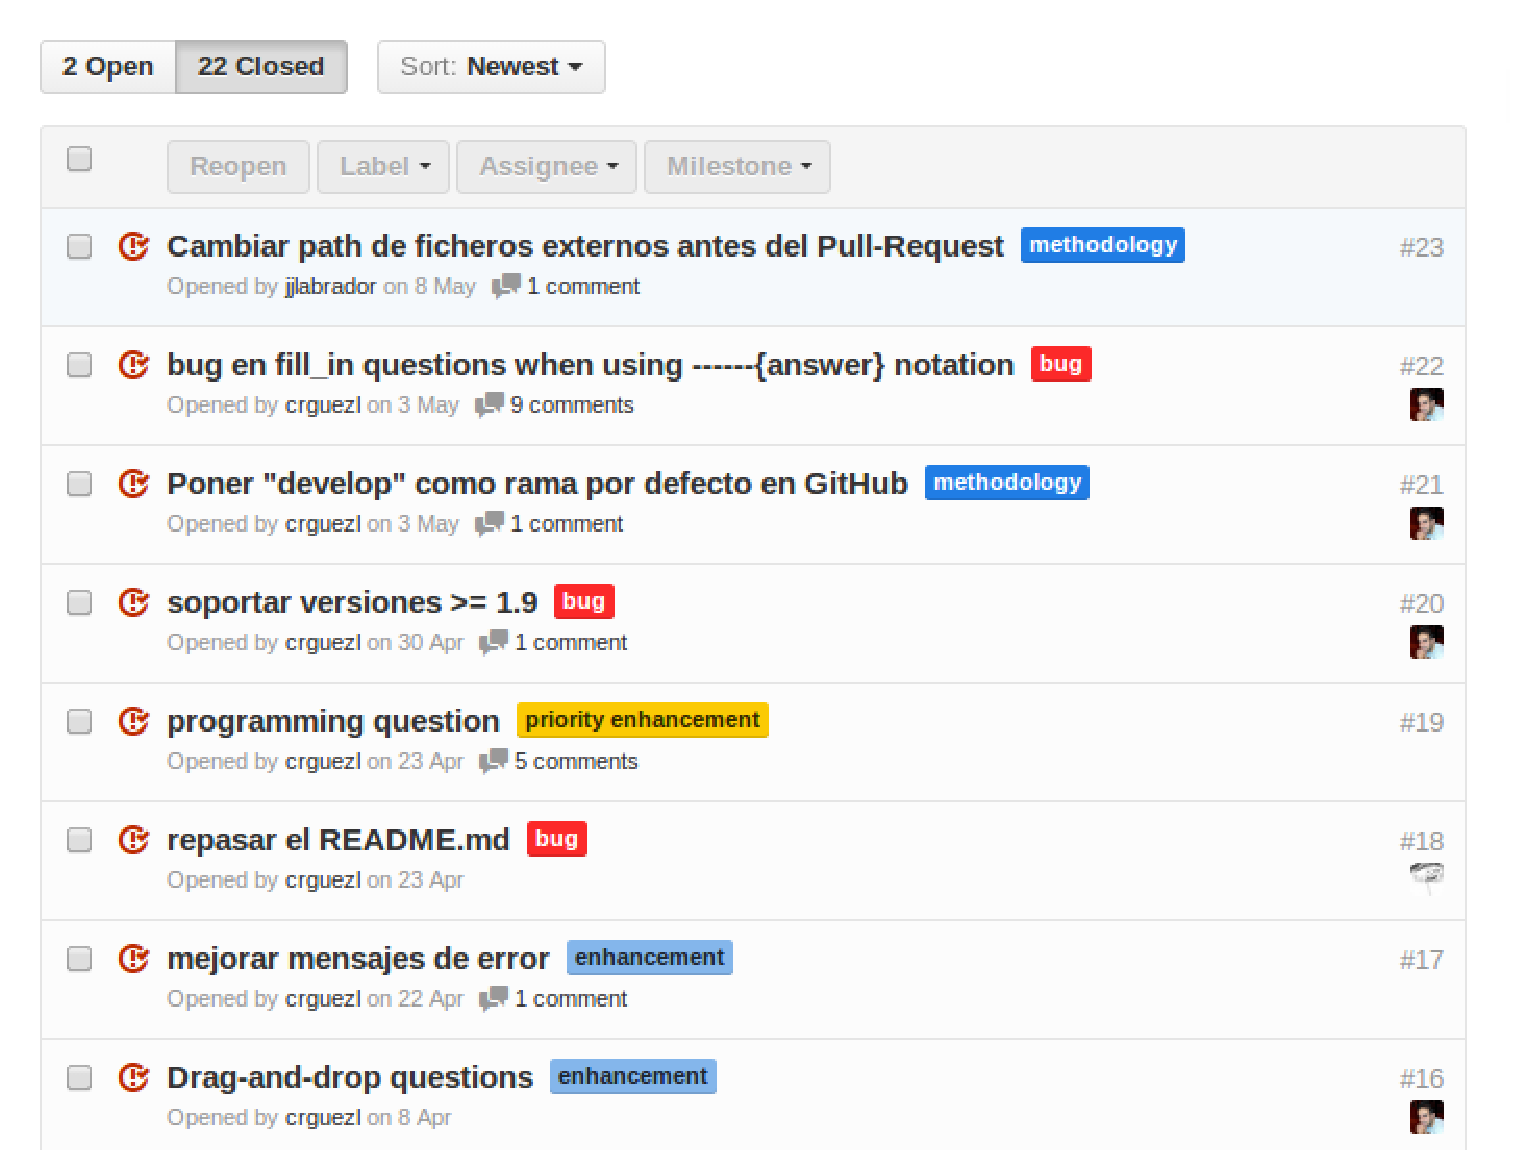
\includegraphics[width=1\textwidth]{images/github4.eps}%
\lthtmlpictureZ
\lthtmlcheckvsize\clearpage}

\stepcounter{subsection}
\stepcounter{subsection}
\stepcounter{section}
\stepcounter{chapter}
\stepcounter{section}
\stepcounter{subsection}
\stepcounter{subsection}
\stepcounter{chapter}
{\newpage\clearpage
\lthtmlpictureA{tex2html_wrap11629}%
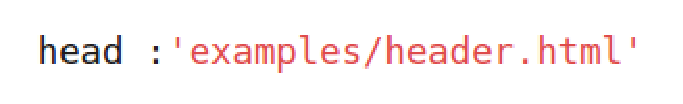
\includegraphics[width=0.4\textwidth]{images/header.eps}%
\lthtmlpictureZ
\lthtmlcheckvsize\clearpage}

{\newpage\clearpage
\lthtmlpictureA{tex2html_wrap11633}%
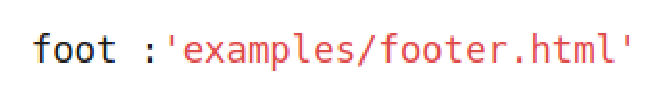
\includegraphics[width=0.4\textwidth]{images/footer.eps}%
\lthtmlpictureZ
\lthtmlcheckvsize\clearpage}

{\newpage\clearpage
\lthtmlpictureA{tex2html_wrap11637}%
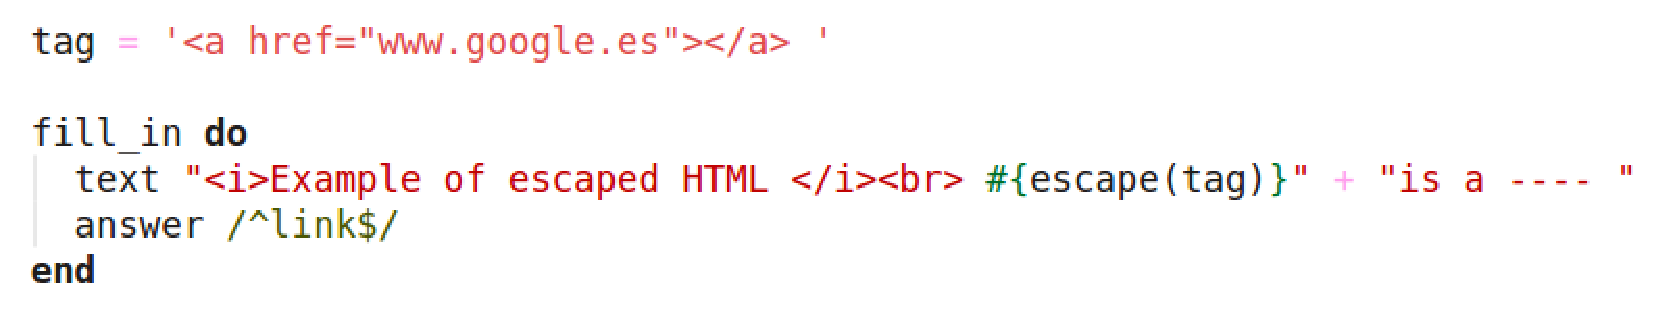
\includegraphics[width=1\textwidth]{images/tag.eps}%
\lthtmlpictureZ
\lthtmlcheckvsize\clearpage}

{\newpage\clearpage
\lthtmlpictureA{tex2html_wrap11641}%
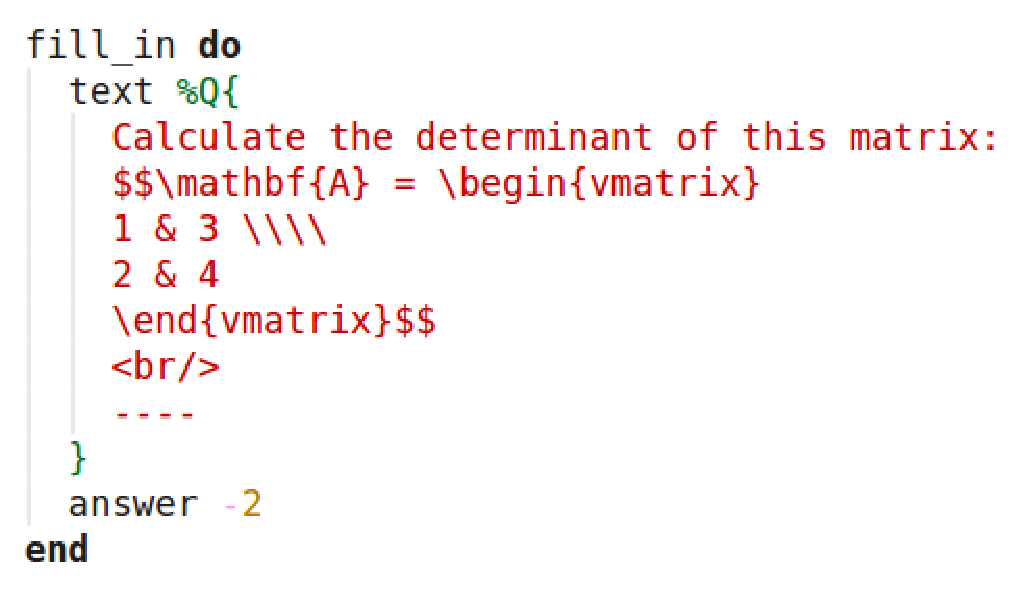
\includegraphics[width=0.6\textwidth]{images/latex.eps}%
\lthtmlpictureZ
\lthtmlcheckvsize\clearpage}

{\newpage\clearpage
\lthtmlpictureA{tex2html_wrap11645}%
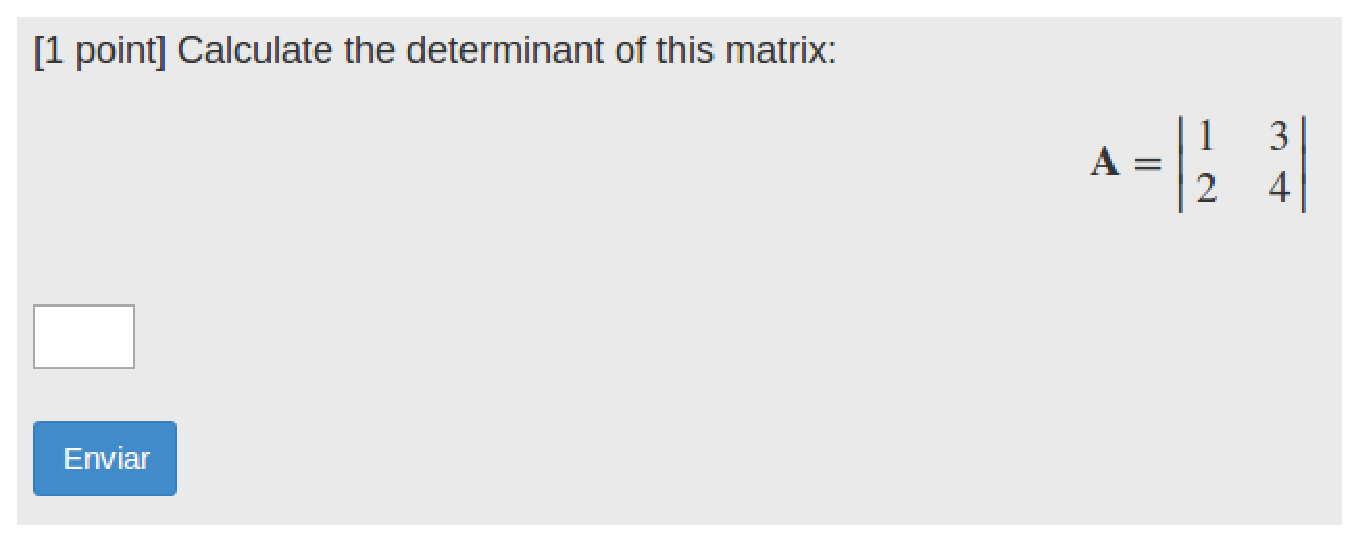
\includegraphics[width=0.8\textwidth]{images/latex2.eps}%
\lthtmlpictureZ
\lthtmlcheckvsize\clearpage}

{\newpage\clearpage
\lthtmlpictureA{tex2html_wrap11649}%
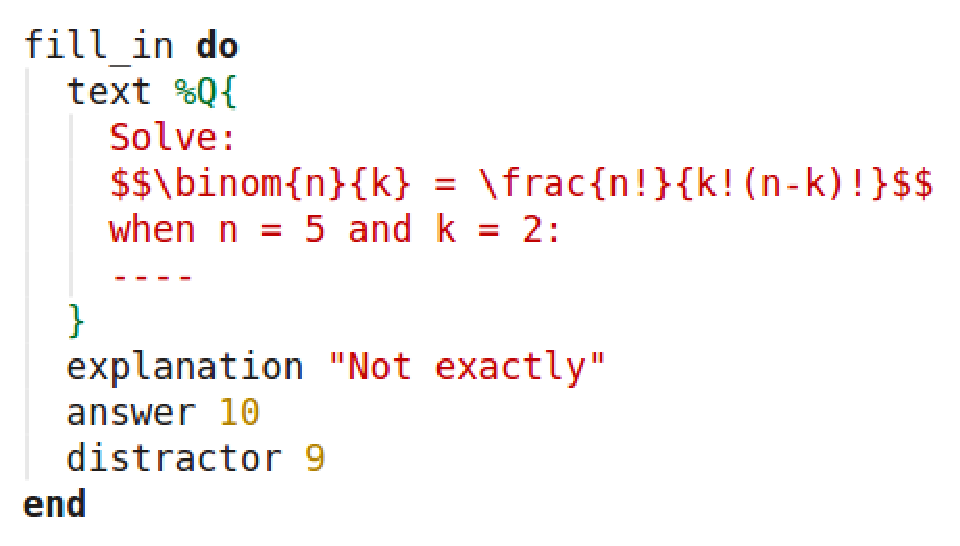
\includegraphics[width=0.6\textwidth]{images/numeric_answer.eps}%
\lthtmlpictureZ
\lthtmlcheckvsize\clearpage}

{\newpage\clearpage
\lthtmlpictureA{tex2html_wrap11653}%
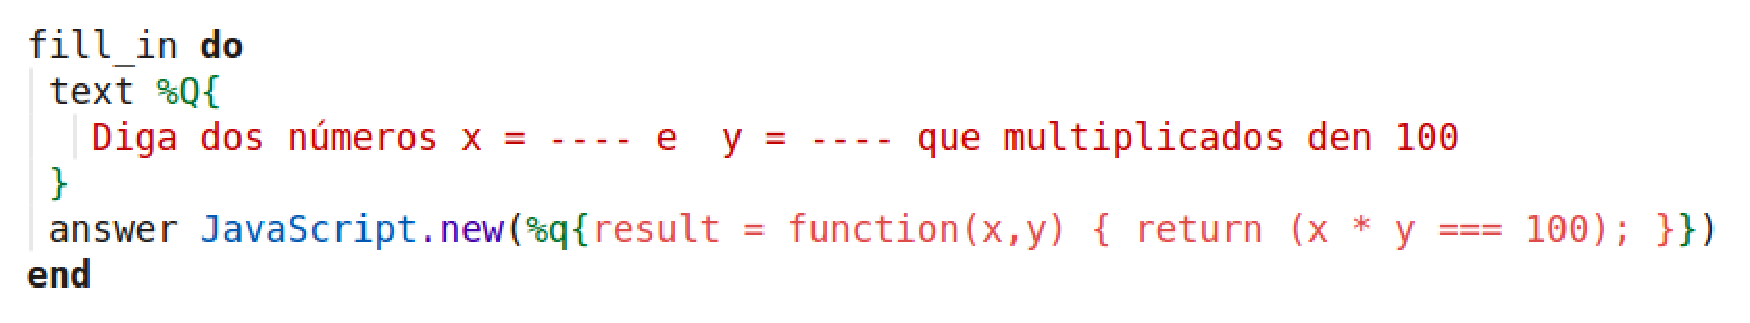
\includegraphics[width=1\textwidth]{images/javascript_answer.eps}%
\lthtmlpictureZ
\lthtmlcheckvsize\clearpage}

{\newpage\clearpage
\lthtmlpictureA{tex2html_wrap11657}%
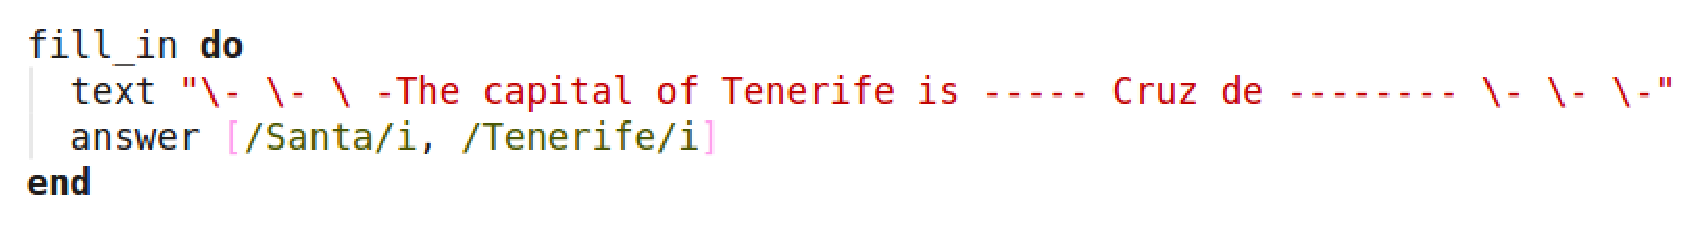
\includegraphics[width=1\textwidth]{images/input.eps}%
\lthtmlpictureZ
\lthtmlcheckvsize\clearpage}

{\newpage\clearpage
\lthtmlpictureA{tex2html_wrap11661}%
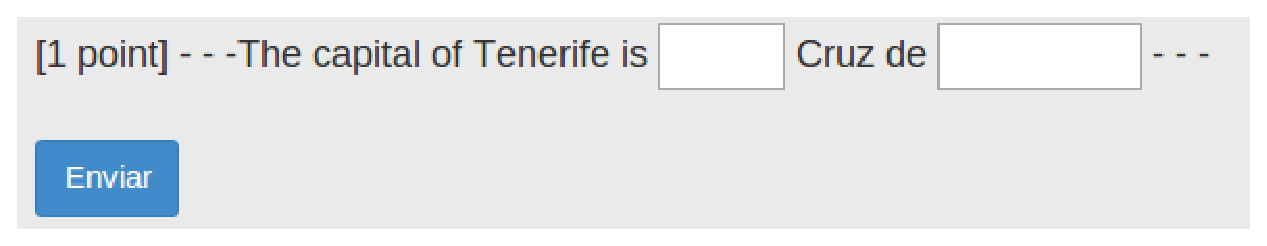
\includegraphics[width=0.8\textwidth]{images/input2.eps}%
\lthtmlpictureZ
\lthtmlcheckvsize\clearpage}

{\newpage\clearpage
\lthtmlpictureA{tex2html_wrap11665}%
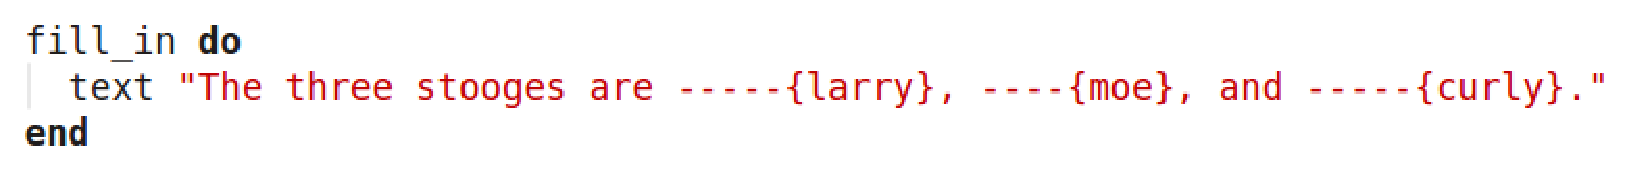
\includegraphics[width=1\textwidth]{images/simplificated1.eps}%
\lthtmlpictureZ
\lthtmlcheckvsize\clearpage}

{\newpage\clearpage
\lthtmlpictureA{tex2html_wrap11669}%
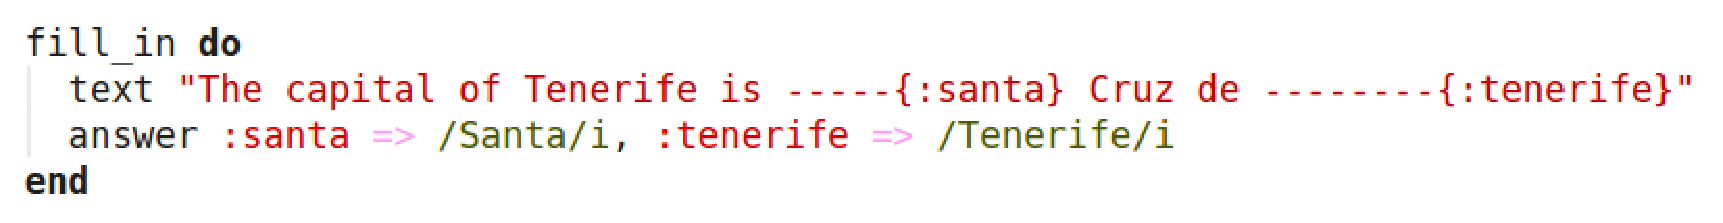
\includegraphics[width=1\textwidth]{images/simplificated2.eps}%
\lthtmlpictureZ
\lthtmlcheckvsize\clearpage}

{\newpage\clearpage
\lthtmlpictureA{tex2html_wrap11673}%
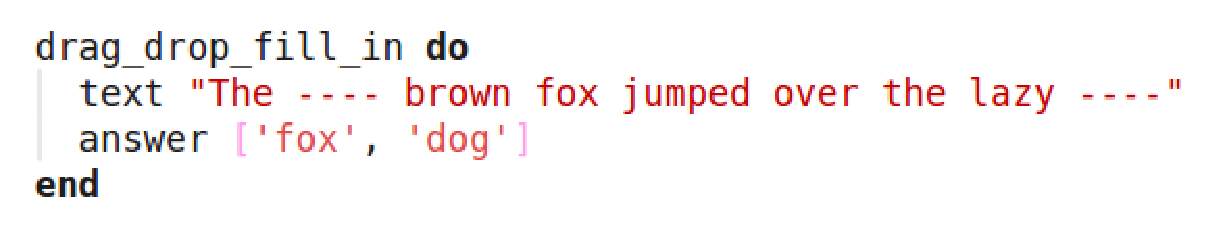
\includegraphics[width=0.8\textwidth]{images/dd1.eps}%
\lthtmlpictureZ
\lthtmlcheckvsize\clearpage}

{\newpage\clearpage
\lthtmlpictureA{tex2html_wrap11677}%
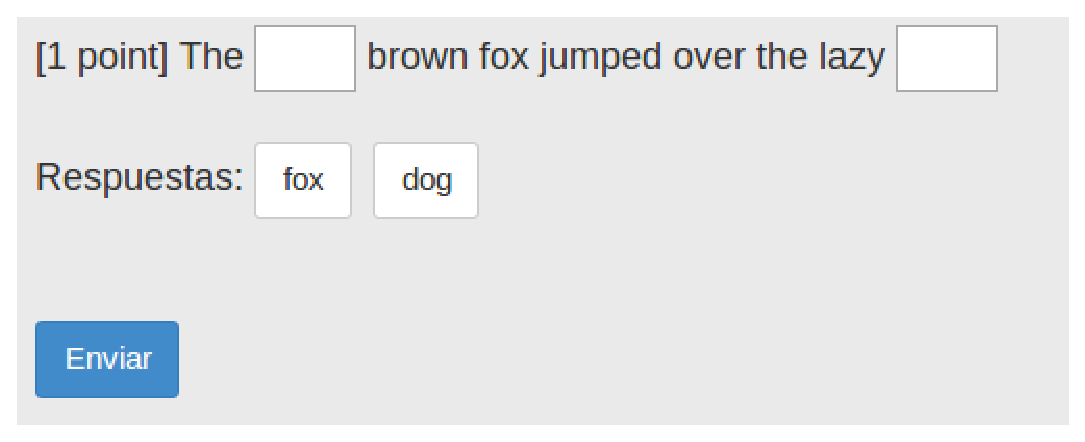
\includegraphics[width=0.8\textwidth]{images/dd1r.eps}%
\lthtmlpictureZ
\lthtmlcheckvsize\clearpage}

{\newpage\clearpage
\lthtmlpictureA{tex2html_wrap11681}%
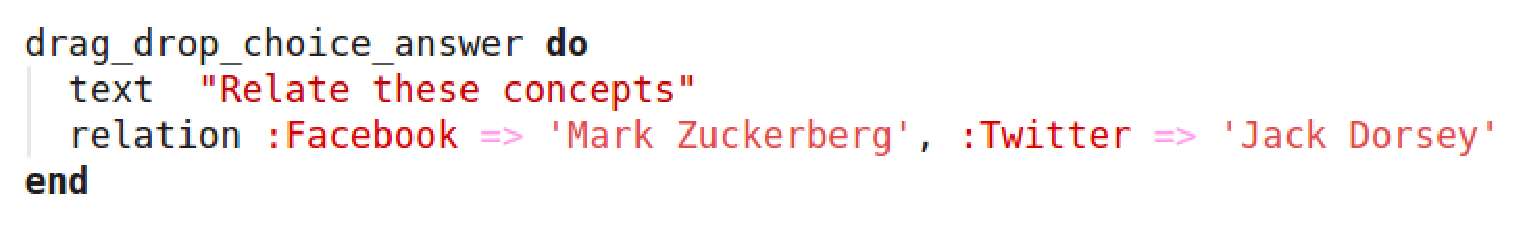
\includegraphics[width=1\textwidth]{images/dd2.eps}%
\lthtmlpictureZ
\lthtmlcheckvsize\clearpage}

{\newpage\clearpage
\lthtmlpictureA{tex2html_wrap11685}%
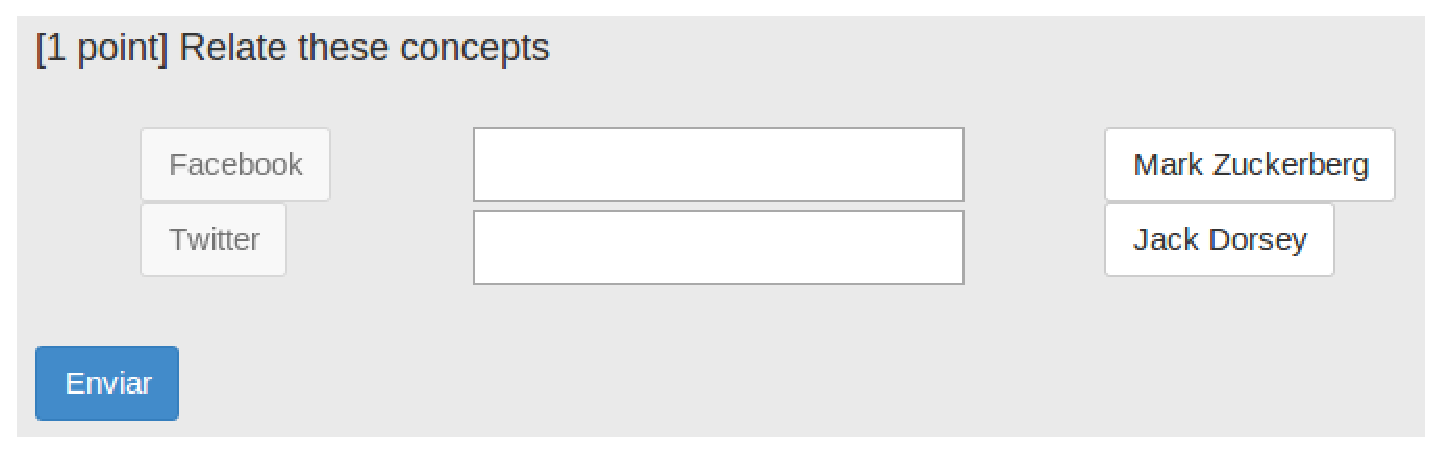
\includegraphics[width=1\textwidth]{images/dd2r.eps}%
\lthtmlpictureZ
\lthtmlcheckvsize\clearpage}

{\newpage\clearpage
\lthtmlpictureA{tex2html_wrap11689}%
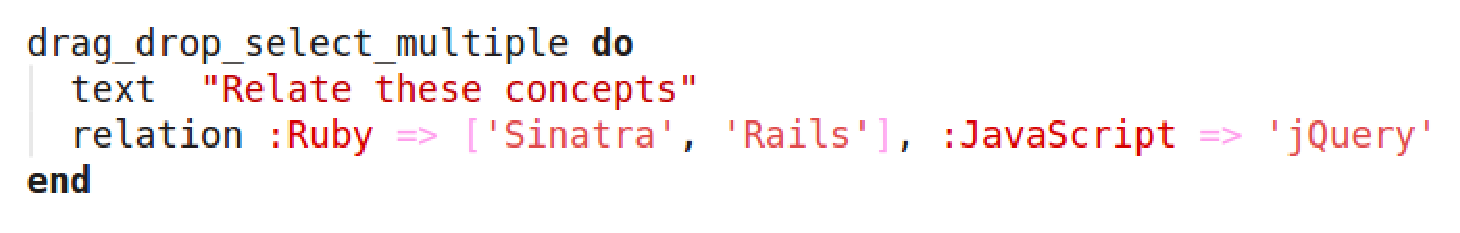
\includegraphics[width=1\textwidth]{images/dd3.eps}%
\lthtmlpictureZ
\lthtmlcheckvsize\clearpage}

{\newpage\clearpage
\lthtmlpictureA{tex2html_wrap11693}%
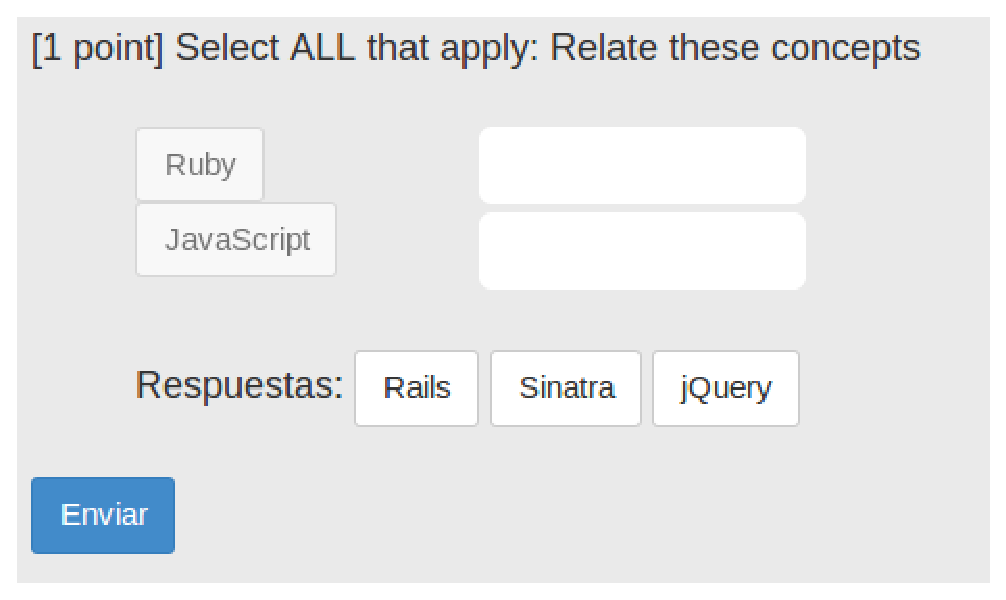
\includegraphics[width=0.6\textwidth]{images/dd3r.eps}%
\lthtmlpictureZ
\lthtmlcheckvsize\clearpage}

{\newpage\clearpage
\lthtmlpictureA{tex2html_wrap11697}%
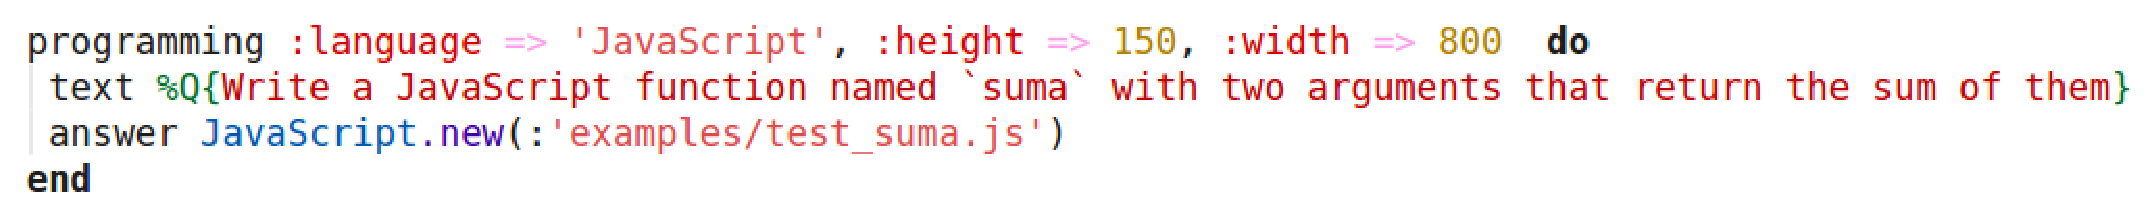
\includegraphics[width=1.1\textwidth,height=0.1\textwidth]{images/programming1.eps}%
\lthtmlpictureZ
\lthtmlcheckvsize\clearpage}

{\newpage\clearpage
\lthtmlpictureA{tex2html_wrap11701}%
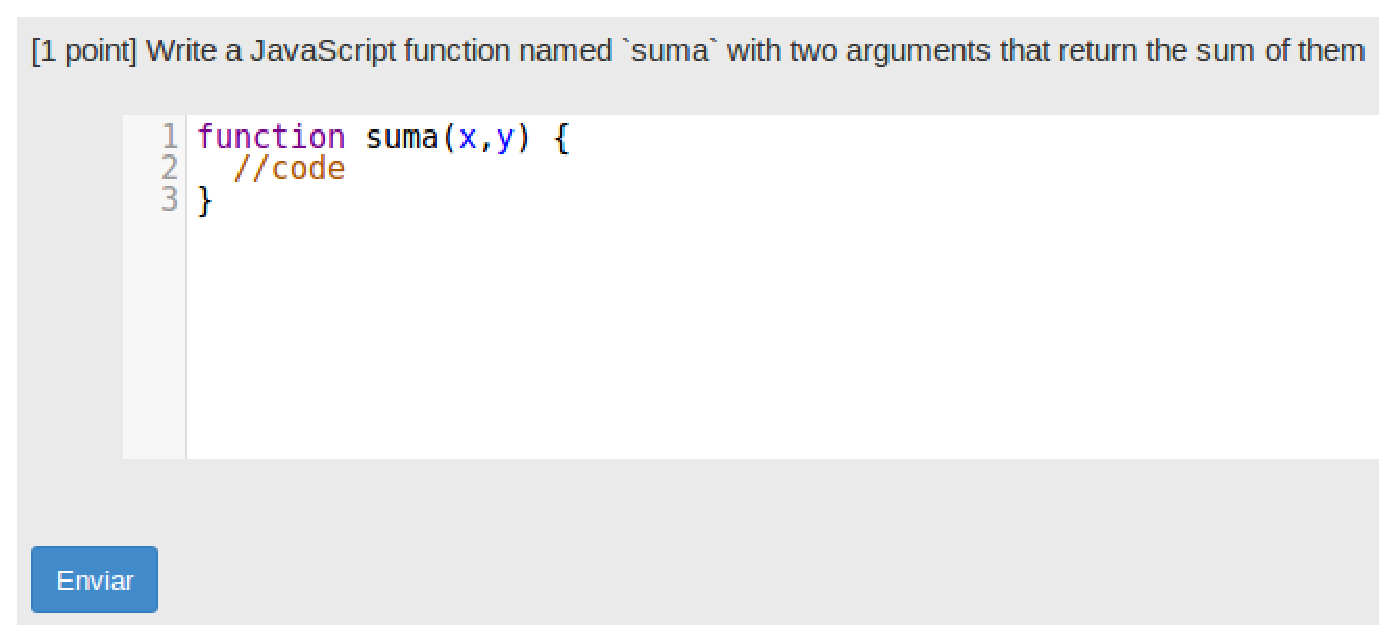
\includegraphics[width=0.9\textwidth]{images/programming1r.eps}%
\lthtmlpictureZ
\lthtmlcheckvsize\clearpage}

{\newpage\clearpage
\lthtmlpictureA{tex2html_wrap11705}%
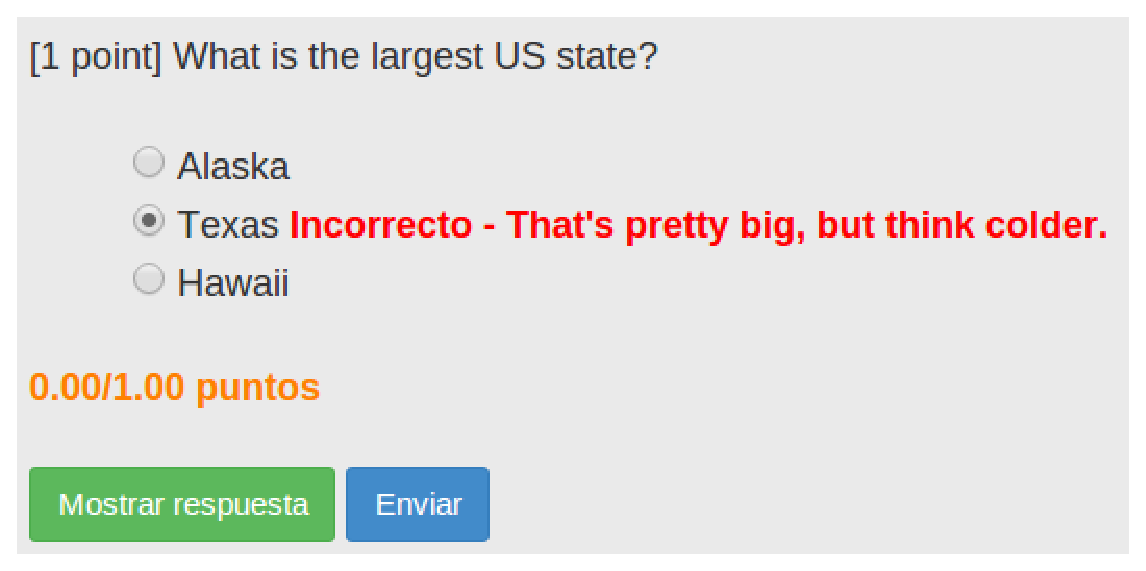
\includegraphics[width=0.7\textwidth]{images/validation1.eps}%
\lthtmlpictureZ
\lthtmlcheckvsize\clearpage}

{\newpage\clearpage
\lthtmlpictureA{tex2html_wrap11709}%

\includegraphics[width=0.9\textwidth]{images/validation2.eps}%
\lthtmlpictureZ
\lthtmlcheckvsize\clearpage}

{\newpage\clearpage
\lthtmlpictureA{tex2html_wrap11713}%
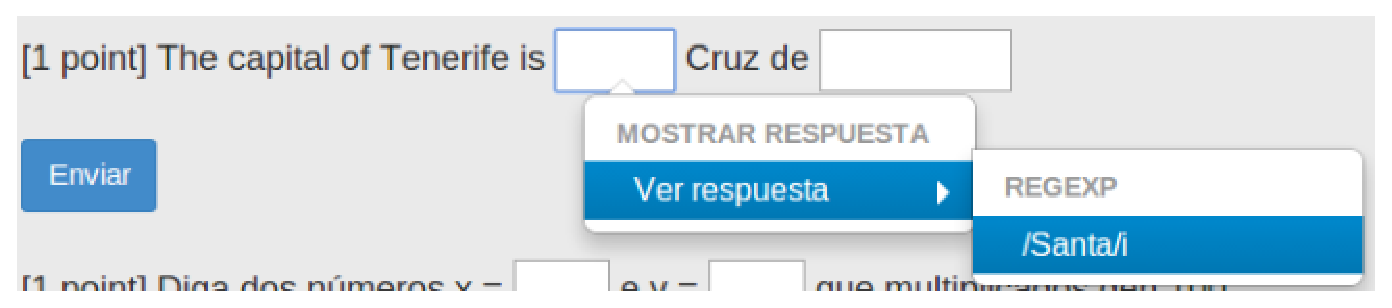
\includegraphics[width=0.8\textwidth]{images/show_answer.eps}%
\lthtmlpictureZ
\lthtmlcheckvsize\clearpage}

{\newpage\clearpage
\lthtmlpictureA{tex2html_wrap11717}%
\includegraphics[width=0.65\textwidth]{images/show_answer1.eps}%
\lthtmlpictureZ
\lthtmlcheckvsize\clearpage}

{\newpage\clearpage
\lthtmlpictureA{tex2html_wrap11721}%
\includegraphics[width=0.7\textwidth]{images/i18n.eps}%
\lthtmlpictureZ
\lthtmlcheckvsize\clearpage}

\stepcounter{section}
\stepcounter{subsection}
\stepcounter{subsection}
\stepcounter{chapter}
{\newpage\clearpage
\lthtmlpictureA{tex2html_wrap11729}%
\includegraphics[width=0.5\textwidth]{images/teachers.eps}%
\lthtmlpictureZ
\lthtmlcheckvsize\clearpage}

{\newpage\clearpage
\lthtmlpictureA{tex2html_wrap11733}%
\includegraphics[width=0.5\textwidth]{images/students.eps}%
\lthtmlpictureZ
\lthtmlcheckvsize\clearpage}

{\newpage\clearpage
\lthtmlpictureA{tex2html_wrap11737}%
\includegraphics[width=0.4\textwidth]{images/config.eps}%
\lthtmlpictureZ
\lthtmlcheckvsize\clearpage}

{\newpage\clearpage
\lthtmlpictureA{tex2html_wrap11741}%
\includegraphics[width=0.4\textwidth]{images/app.eps}%
\lthtmlpictureZ
\lthtmlcheckvsize\clearpage}

\stepcounter{section}
\stepcounter{subsection}
\stepcounter{subsection}
\stepcounter{subsection}
\stepcounter{chapter}
\stepcounter{chapter}
\stepcounter{chapter}
\stepcounter{section}
\stepcounter{section}
\stepcounter{section}
\stepcounter{section}
\stepcounter{section}
\stepcounter{chapter}
\stepcounter{chapter}
\stepcounter{section}
{\newpage\clearpage
\lthtmlfigureA{lstlisting3940}%
\begin{lstlisting}
<html>
  <head>
    <meta charset="utf-8">
    <meta http-equiv="X-UA-Compatible" content="IE=edge">
    <meta name="viewport" content="width=device-width, initial-scale=1">
    <title><%= quiz.title %></title>
    <!-- Bootstrap CSS -->
    <%= @bootstrap_css %>
    <style type="text/css" media="all">
      /* Custom CSS */
      /* ...........*/
      /* Inputs size */
      <%= @sass %>
    </style>
    <!-- jQuery ContextMenu CSS -->
    <%= @context_menu_css %>
    <!-- Any CSS included by the user -->
    <%= @css_custom %>
    <!-- Mathjax -->
    <%= @mathjax %>
    <!-- CodeMirror -->
    <%= @codemirror %>
  </head>
  <body>
   <div class="container">
      <% if (quiz.get_header)%>
          <h3><%= quiz.title %></h3>
          <%= quiz.get_header %>
          <br></br>
      <% else %>
        <!-- HTML Code -->
      <% end %>
      <%= yield %>
      <% if (quiz.get_footer) %>
        <%= quiz.get_footer %>
        <br></br>
      <% else %>
        <!-- HTML Code -->
      <% end %>
    </div>
    <!-- #### JavaScripts #### -->
    <!-- jQuery -->
    <%= @jQuery %>
    <!-- Internationalization -->
    <%= @i18n %>
    <!-- Drag and Drop -->
    <%= @dragdrop %>
    <!-- XRegexp -->
    <%= @xregexp %>
    <!-- Form validation -->
    <%= @validation_js %>
    <!-- jQuery ContextMenu -->
    <%= @context_menu %>
    <!-- Any JavaScript included by the user -->
    <%= @js_custom %>
    <!-- CodeMirror object -->
    <%= @codemirror_object %>
    <!-- JavaScript for Bootstrap -->
    <%= @bootstrap_js %>
  </body>
</html>
\end{lstlisting}%
\lthtmlfigureZ
\lthtmlcheckvsize\clearpage}

\stepcounter{section}
{\newpage\clearpage
\lthtmlfigureA{lstlisting3946}%
\begin{lstlisting}
quiz 'Example quiz' do
  head :'examples/header.html'  # Opcional
\par
# Preguntas
\par
foot :'examples/footer.html'  # Opcional
end
\end{lstlisting}%
\lthtmlfigureZ
\lthtmlcheckvsize\clearpage}

\stepcounter{subsection}
{\newpage\clearpage
\lthtmlfigureA{lstlisting3953}%
\begin{lstlisting}
tag = '<a href="www.google.es"></a> '
fill_in do
  text "<i>Example of escaped HTML and three hyphens not evaluated:</i><br> 
  #{escape(tag)}" + "is a \\-\\-\\- ---- " + '\-\-\-'
  answer /^link$/
end
\end{lstlisting}%
\lthtmlfigureZ
\lthtmlcheckvsize\clearpage}

{\newpage\clearpage
\lthtmlfigureA{lstlisting3957}%
\begin{lstlisting}
fill_in :points => 2 do
  text 'The visionary founder of Apple is --------'
  comment 'Question too easy'
  answer /^ste(ve|phen)\s+jobs #comment $/imx
  distractor /^steve\s+wozniak/i, :explanation => 'Almost, but not quite.'
end
\end{lstlisting}%
\lthtmlfigureZ
\lthtmlcheckvsize\clearpage}

{\newpage\clearpage
\lthtmlfigureA{lstlisting3960}%
\begin{lstlisting}
fill_in do
  text %q{
    When x = 2, the solution of $\sqrt{3x+3}+(1+x)^2$\  is:
    ----
\par
answer 12
  distractor 11, :explanation => "Try again!"
end
\end{lstlisting}%
\lthtmlfigureZ
\lthtmlcheckvsize\clearpage}

{\newpage\clearpage
\lthtmlfigureA{lstlisting3965}%
\begin{lstlisting}
fill_in do
  text 'The ---- brown fox jumped over the lazy ----'
  answer [/fox/, /dog/]
end
\end{lstlisting}%
\lthtmlfigureZ
\lthtmlcheckvsize\clearpage}

{\newpage\clearpage
\lthtmlfigureA{lstlisting3969}%
\begin{lstlisting}
fill_in do
  text 'The ---- brown fox jumped over the lazy ----'
  answer [/fox/, /dog/], :order => false
end
\end{lstlisting}%
\lthtmlfigureZ
\lthtmlcheckvsize\clearpage}

{\newpage\clearpage
\lthtmlfigureA{lstlisting3975}%
\begin{lstlisting}
fill_in do
  text 'The three stooges are -----{larry}, ----{moe}, and -----{curly}.'
end
\end{lstlisting}%
\lthtmlfigureZ
\lthtmlcheckvsize\clearpage}

{\newpage\clearpage
\lthtmlfigureA{lstlisting3981}%
\begin{lstlisting}
fill_in do
  text "The capital of Tenerife is -----{:santa} Cruz de --------{:tenerife}"
  answer :santa => /Santa/i, :tenerife => /Tenerife/i
end
\end{lstlisting}%
\lthtmlfigureZ
\lthtmlcheckvsize\clearpage}

{\newpage\clearpage
\lthtmlfigureA{lstlisting3988}%
\begin{lstlisting}
fill_in do
  text %q{
    Diga dos numeros x = ---- e  y = ---- que multiplicados den 100
\par
answer JavaScript.new(%q{result = function(x,y) { return (x * y === 100); }})
end
\end{lstlisting}%
\lthtmlfigureZ
\lthtmlcheckvsize\clearpage}

\stepcounter{subsection}
{\newpage\clearpage
\lthtmlfigureA{lstlisting3993}%
\begin{lstlisting}
drag_drop_fill_in do
  text 'The ---- brown fox jumped over the lazy ----'
  answer ['fox', 'dog']
end
\end{lstlisting}%
\lthtmlfigureZ
\lthtmlcheckvsize\clearpage}

\stepcounter{subsection}
{\newpage\clearpage
\lthtmlfigureA{lstlisting3999}%
\begin{lstlisting}
choice_answer :randomize => true do
  text  "What is the largest US state?"
  explanation "Not big enough." # for distractors without their own explanation
  answer 'Alaska'
  distractor 'Hawaii'
  distractor 'Texas', :explanation => "That's pretty big, but think colder."
end
\end{lstlisting}%
\lthtmlfigureZ
\lthtmlcheckvsize\clearpage}

\stepcounter{subsection}
{\newpage\clearpage
\lthtmlfigureA{lstlisting4004}%
\begin{lstlisting}
truefalse 'The earth is flat.', false, :explanation => 'No, just looks that way'
\end{lstlisting}%
\lthtmlfigureZ
\lthtmlcheckvsize\clearpage}

\stepcounter{subsection}
{\newpage\clearpage
\lthtmlfigureA{lstlisting4010}%
\begin{lstlisting}
drag_drop_choice_answer do
  text  "Relate these concepts"
  relation :Facebook => 'Mark Zuckerberg', :Twitter => 'Jack Dorsey'
end
\end{lstlisting}%
\lthtmlfigureZ
\lthtmlcheckvsize\clearpage}

\stepcounter{subsection}
{\newpage\clearpage
\lthtmlfigureA{lstlisting4015}%
\begin{lstlisting}
select_multiple do
  text "Which are American political parties?"
  answer "Democrats"
  answer "Republicans"
  answer "Greens", :explanation => "Yes, they're a party!"
  distractor "Tories", :explanation => "They're British"
  distractor "Social Democrats"
end
\end{lstlisting}%
\lthtmlfigureZ
\lthtmlcheckvsize\clearpage}

\stepcounter{subsection}
{\newpage\clearpage
\lthtmlfigureA{lstlisting4019}%
\begin{lstlisting}
drag_drop_select_multiple do
  text  "Relate these concepts"
  relation :Ruby => ['Sinatra', 'Rails'], :JavaScript => 'jQuery'
end
\end{lstlisting}%
\lthtmlfigureZ
\lthtmlcheckvsize\clearpage}

\stepcounter{subsection}
{\newpage\clearpage
\lthtmlfigureA{lstlisting4036}%
\begin{lstlisting}
programming :language => 'JavaScript', :height => 150, :width => 800  do
  text %q{Write a JavaScript function named `suma` with two arguments that
  return the sum of them
  answer JavaScript.new(:'examples/test_suma.js')
end
\end{lstlisting}%
\lthtmlfigureZ
\lthtmlcheckvsize\clearpage}

\stepcounter{subsection}
\stepcounter{subsection}
\stepcounter{section}
\stepcounter{subsection}
{\newpage\clearpage
\lthtmlfigureA{lstlisting4058}%
\begin{lstlisting}
fill_in do
  text %q{
    Diga dos numeros x = ---- e  y = ---- que multiplicados den 100
\par
answer Ruby.new(%q{Proc.new do |x,y| x * y == 100 end})
end
\end{lstlisting}%
\lthtmlfigureZ
\lthtmlcheckvsize\clearpage}

\stepcounter{subsection}
{\newpage\clearpage
\lthtmlfigureA{lstlisting4062}%
\begin{lstlisting}
programming :language => 'Ruby', :height => 150, :width => 800  do
  text %q{Write a Ruby function named `suma` with two arguments that 
  return the sum of them
  answer Ruby.new(:'examples/test_suma.rb')
end
\end{lstlisting}%
\lthtmlfigureZ
\lthtmlcheckvsize\clearpage}

\stepcounter{subsection}
{\newpage\clearpage
\lthtmlfigureA{lstlisting4069}%
\begin{lstlisting}
  quiz 'Example quiz' do
\par
teachers 'jjlabradorglez@gmail.com'
\par
.
    .
    .
  end
  \end{lstlisting}%
\lthtmlfigureZ
\lthtmlcheckvsize\clearpage}

{\newpage\clearpage
\lthtmlfigureA{lstlisting4072}%
\begin{lstlisting}
  quiz 'Example quiz' do
\par
students :'jjlabradorglez@gmail.com' => {:surname => 'Labrador Gonzalez', 
               :name => 'Juan Jose'}, 
             :'tutu@gmail.com' => {:surname => 'Chuchu', :name => 'Tutu'}
    .
    .
    .
  end
  \end{lstlisting}%
\lthtmlfigureZ
\lthtmlcheckvsize\clearpage}

{\newpage\clearpage
\lthtmlfigureA{lstlisting4078}%
\begin{lstlisting}
  quiz 'Example quiz' do
\par
students :'examples/students.csv''
\par
.
    .
    .
  end
  \end{lstlisting}%
\lthtmlfigureZ
\lthtmlcheckvsize\clearpage}

{\newpage\clearpage
\lthtmlpictureA{tex2html_wrap11939}%
\includegraphics[width=1.2\textwidth]{images/config_yml.eps}%
\lthtmlpictureZ
\lthtmlcheckvsize\clearpage}

{\newpage\clearpage
\lthtmlfigureA{lstlisting4102}%
\begin{lstlisting}
  quiz 'Example quiz' do
\par
.
    .
\par
config :'examples/config.yml'
    .
    .
  end
\end{lstlisting}%
\lthtmlfigureZ
\lthtmlcheckvsize\clearpage}

\stepcounter{subsection}
{\newpage\clearpage
\lthtmlpictureA{tex2html_wrap11944}%
\includegraphics[width=0.5\textwidth]{images/gdc0.eps}%
\lthtmlpictureZ
\lthtmlcheckvsize\clearpage}

{\newpage\clearpage
\lthtmlpictureA{tex2html_wrap11948}%
\includegraphics[width=0.7\textwidth]{images/gdc1.eps}%
\lthtmlpictureZ
\lthtmlcheckvsize\clearpage}

{\newpage\clearpage
\lthtmlpictureA{tex2html_wrap11952}%
\includegraphics[width=0.3\textwidth]{images/gdc2.eps}%
\lthtmlpictureZ
\lthtmlcheckvsize\clearpage}

{\newpage\clearpage
\lthtmlpictureA{tex2html_wrap11956}%
\includegraphics[width=0.3\textwidth]{images/gdc3.eps}%
\lthtmlpictureZ
\lthtmlcheckvsize\clearpage}

{\newpage\clearpage
\lthtmlpictureA{tex2html_wrap11960}%
\includegraphics[width=0.5\textwidth]{images/gdc4.eps}%
\lthtmlpictureZ
\lthtmlcheckvsize\clearpage}

{\newpage\clearpage
\lthtmlpictureA{tex2html_wrap11964}%
\includegraphics[width=0.7\textwidth]{images/gdc5.eps}%
\lthtmlpictureZ
\lthtmlcheckvsize\clearpage}

{\newpage\clearpage
\lthtmlpictureA{tex2html_wrap11968}%
\includegraphics[width=1.2\textwidth]{images/gdc6.eps}%
\lthtmlpictureZ
\lthtmlcheckvsize\clearpage}

\stepcounter{subsection}
\stepcounter{subsection}
\stepcounter{subsection}
{\newpage\clearpage
\lthtmlpictureA{tex2html_wrap11975}%
\includegraphics[width=0.9\textwidth]{images/app1.eps}%
\lthtmlpictureZ
\lthtmlcheckvsize\clearpage}

{\newpage\clearpage
\lthtmlpictureA{tex2html_wrap11979}%
\includegraphics[width=0.9\textwidth]{images/app2.eps}%
\lthtmlpictureZ
\lthtmlcheckvsize\clearpage}

{\newpage\clearpage
\lthtmlpictureA{tex2html_wrap11983}%
\includegraphics[width=0.9\textwidth]{images/app3.eps}%
\lthtmlpictureZ
\lthtmlcheckvsize\clearpage}

{\newpage\clearpage
\lthtmlpictureA{tex2html_wrap11987}%
\includegraphics[width=0.75\textwidth]{images/app4.eps}%
\lthtmlpictureZ
\lthtmlcheckvsize\clearpage}

{\newpage\clearpage
\lthtmlpictureA{tex2html_wrap11991}%
\includegraphics[width=0.6\textwidth]{images/app5.eps}%
\lthtmlpictureZ
\lthtmlcheckvsize\clearpage}

{\newpage\clearpage
\lthtmlpictureA{tex2html_wrap11995}%
\includegraphics[width=0.75\textwidth]{images/app6.eps}%
\lthtmlpictureZ
\lthtmlcheckvsize\clearpage}

{\newpage\clearpage
\lthtmlpictureA{tex2html_wrap11999}%
\includegraphics[width=0.8\textwidth]{images/app7.eps}%
\lthtmlpictureZ
\lthtmlcheckvsize\clearpage}

{\newpage\clearpage
\lthtmlpictureA{tex2html_wrap12003}%
\includegraphics[width=1\textwidth]{images/app8.eps}%
\lthtmlpictureZ
\lthtmlcheckvsize\clearpage}

{\newpage\clearpage
\lthtmlpictureA{tex2html_wrap12007}%
\includegraphics[width=0.8\textwidth]{images/app9.eps}%
\lthtmlpictureZ
\lthtmlcheckvsize\clearpage}

{\newpage\clearpage
\lthtmlpictureA{tex2html_wrap12011}%
\includegraphics[width=0.6\textwidth]{images/app10.eps}%
\lthtmlpictureZ
\lthtmlcheckvsize\clearpage}

{\newpage\clearpage
\lthtmlpictureA{tex2html_wrap12015}%
\includegraphics[width=1.1\textwidth]{images/app11.eps}%
\lthtmlpictureZ
\lthtmlcheckvsize\clearpage}

{\newpage\clearpage
\lthtmlpictureA{tex2html_wrap12019}%
\includegraphics[width=1.1\textwidth]{images/app12.eps}%
\lthtmlpictureZ
\lthtmlcheckvsize\clearpage}

{\newpage\clearpage
\lthtmlpictureA{tex2html_wrap12023}%
\includegraphics[width=0.8\textwidth]{images/app13.eps}%
\lthtmlpictureZ
\lthtmlcheckvsize\clearpage}

{\newpage\clearpage
\lthtmlpictureA{tex2html_wrap12027}%
\includegraphics[width=1\textwidth]{images/app14.eps}%
\lthtmlpictureZ
\lthtmlcheckvsize\clearpage}

{\newpage\clearpage
\lthtmlpictureA{tex2html_wrap12031}%
\includegraphics[width=0.8\textwidth]{images/app15.eps}%
\lthtmlpictureZ
\lthtmlcheckvsize\clearpage}

{\newpage\clearpage
\lthtmlpictureA{tex2html_wrap12035}%
\includegraphics[width=1.1\textwidth]{images/app16.eps}%
\lthtmlpictureZ
\lthtmlcheckvsize\clearpage}

{\newpage\clearpage
\lthtmlpictureA{tex2html_wrap12039}%
\includegraphics[width=0.6\textwidth]{images/app17.eps}%
\lthtmlpictureZ
\lthtmlcheckvsize\clearpage}

{\newpage\clearpage
\lthtmlpictureA{tex2html_wrap12043}%
\includegraphics[width=1\textwidth]{images/app18.eps}%
\lthtmlpictureZ
\lthtmlcheckvsize\clearpage}

\stepcounter{subsection}

\end{document}
